\documentclass[a4paper,11pt,UTF8]{article}
\usepackage{ctex}
\usepackage{amsmath,amsthm,amssymb,amsfonts}
\usepackage{amsmath}
\usepackage[a4paper]{geometry}
\usepackage{graphicx}
\usepackage{microtype}
\usepackage{siunitx}
\usepackage{booktabs}
\usepackage[colorlinks=false, pdfborder={0 0 0}]{hyperref}
\usepackage{cleveref}
\usepackage{esint} 
\usepackage{graphicx}
\usepackage{ragged2e}
\usepackage{pifont}
\usepackage{extarrows}
\usepackage{mathptmx}
\usepackage{float}
\usepackage{caption}
\usepackage{multirow}
\usepackage{subfigure}
\usepackage{titlesec}
\usepackage{makecell}
\usepackage{tabularx}
\usepackage{graphicx}

\numberwithin{equation}{subsection}

\titleformat{\section}{\Large\bfseries}{\thesection}{1em}{}
\titleformat{\subsection}{\large\bfseries}{\thesubsection}{1em}{}
\titleformat{\subsubsection}{\normalsize\bfseries}{\thesubsubsection}{1em}{}
\begin{document}
\title{\huge 实验报告 \\ 共源放大电路设计、仿真与实现}
\author{电子信息与通信学院 \\ 提高2301班 \\ 张禹阳 \ U202314270}

\maketitle

\begin{figure}[H]
	\centering
	\subfigure{
		
\includegraphics[scale=1]{hust.png}
	}
	\subfigure{
		
\includegraphics[scale=1]{eic.png}
	}
\end{figure}

\tableofcontents\newpage

\section{实验目的}
\begin{itemize}
	\item 学习共源放大电路工作原理
	\item 掌握金属-氧化物-半导体场效应管的主要性能参数及其测试方法
	\item 掌握共源放大电路参数调整方法
	\item 掌握共源放大电路的基本原理与参数测量方法
	\item 掌握MOSFET共源极放大电路的安装与测试 技术
	\item 掌握Multisim软件的使用,实现共源放大电路的仿真实现
\end{itemize}

\section{实验元器件}
\begin{table}[h]
	\centering
	\begin{tabular}{|c|c|c|}
		\hline
		名称 & 型号/参数 & 数量\\
		\hline
		场效应管 & 2N7000 & 1\\
		\hline
		\multirow{3}{*}{电容} & 4.7μF & 1 \\
		\cline{2-3}
		 & 47μF & 1\\
		\cline{2-3}
		 & 1μF & 1\\
		\hline
		电位器 & 500kΩ & 1\\
		\hline
		\multirow{4}{*}{电阻} & 100kΩ & 2 \\
		\cline{2-3}
		 & 5.1kΩ & 1\\
		\cline{2-3}
		 & 51kΩ & 1\\
		\cline{2-3}
 		 & 1kΩ & 1\\
		\hline 		
	\end{tabular}
\end{table}

\section{实验任务}
\begin{enumerate}
	\item MOSFET输出特性曲线仿真
	\item MOSFET转移特性曲线仿真
	\item MOSFET共源放大电路安装、调试及测试
	\item MOSFET共源放大电路仿真
\end{enumerate}

\section{实验原理}
\subsection{MOSFET共源放大电路安装、调试及测试}


图 3.3.6 为 N 沟道增强型 MOSFET 共源极放大电路,其静态工作点可由式(4.3.1) 估算
\begin{subequations}\begin{align}
		V_{\mathrm{GSQ}}=\frac{R_{\mathrm{g2}}}{R_{\mathrm{g1}}+R_{\mathrm{g2}}}\times V_{\mathrm{DD}}-I_{\mathrm{DQ}}R_{\mathrm{s}}  \\
		I_{\mathrm{DQ}}=K_{\mathrm{n}}\left(V_{\mathrm{GS}}-V_{\mathrm{TN}}\right)^{2} \\
		V_{\mathrm{DSQ}}=V_{\mathrm{DD}}-I_{\mathrm{DQ}}(R_{\mathrm{d}}+R_{\mathrm{s}}) 
\end{align}\end{subequations}
动态性能指标可由式(4.1) 估算
\begin{subequations}\begin{align}
		A_\mathrm{v}=-g_\mathrm{m}R_\mathrm{d}\\
		R_{\mathrm{i}}=R_{\mathrm{g1}}//R_{\mathrm{g2}}\\
		R_{\mathrm{o}}=R_{\mathrm{d}}
\end{align}\end{subequations}

\begin{figure}[H]
	\centering
	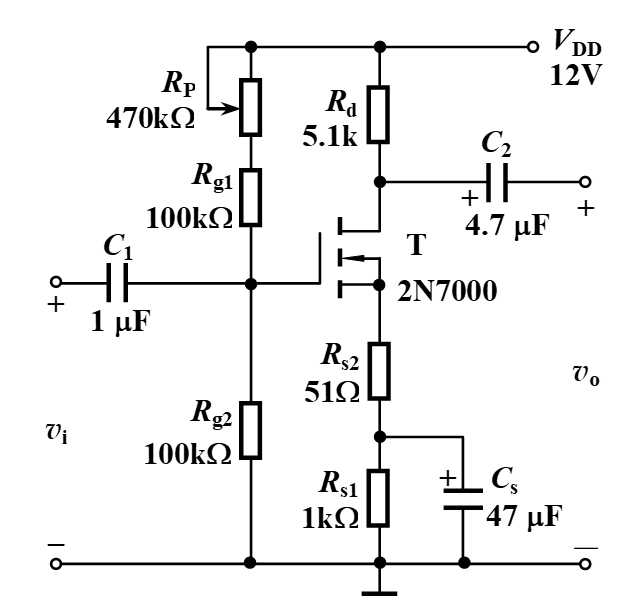
\includegraphics[width=0.7\textwidth]{2.1.png}
	\caption{共源极放大电路}
\end{figure}


数据手册通常会给出$\nu_\mathrm{TN}$和某工作点下的$g_\mathrm{m}$。由表 3.3.1 看出,对于 MOS 管 2N7000,$I_{\mathrm{D} }= 200$mA 时,$g_m^{\prime}= 100$mS, 可得 $K_n= ( g_m^{\prime}/2) ^2/I_{\mathrm{D} }= 12.5$mA$/V^2$ 式(3.3.4a)中的$g_\mathrm{m}$是图 3.3.6 电路静态工作点下 MOS 管的互导,同样可得
\begin{align}
	g_m&=g_m'\sqrt{I_{\mathrm{DQ}}/I_{\mathrm{D}}}\\
	g_{\mathrm{m}}&=10\sqrt{I_{\mathrm{DQ}}/2}\mathrm{mS}
\end{align}

由数据表可知$V_{\mathrm{TN}}$在0.8-3V之间,这里取 $V_{\mathrm{TN}}=1.75\mathrm{V}$

\section{实验过程}

\subsection{Multisim 仿真}

\subsubsection{DC Operating Point 模拟直流静态工作点}
电路图如下:
\begin{figure}[H]
	\centering
	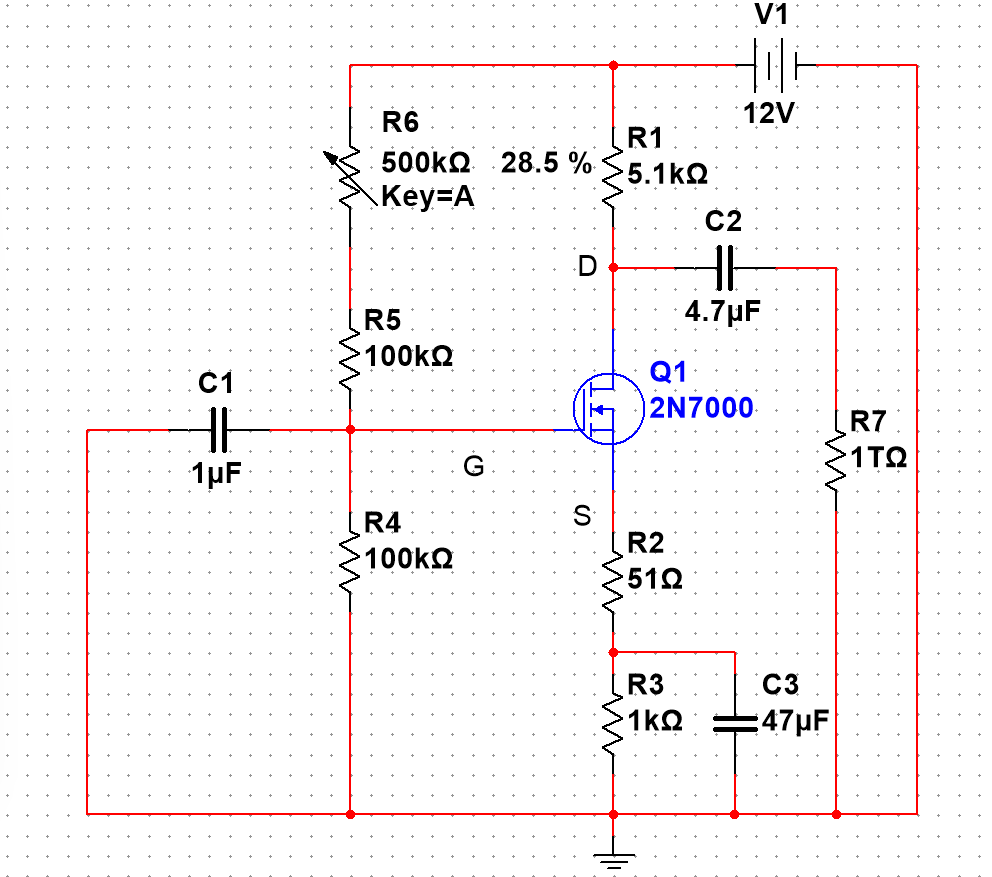
\includegraphics[width=0.7\textwidth]{2.2.png}
	\caption{模拟直流静态工作点电路}
\end{figure}

测量静态工作点,选择直流工作点分析,得到此时对应的直流工作点:
\begin{figure}[H]
	\centering
	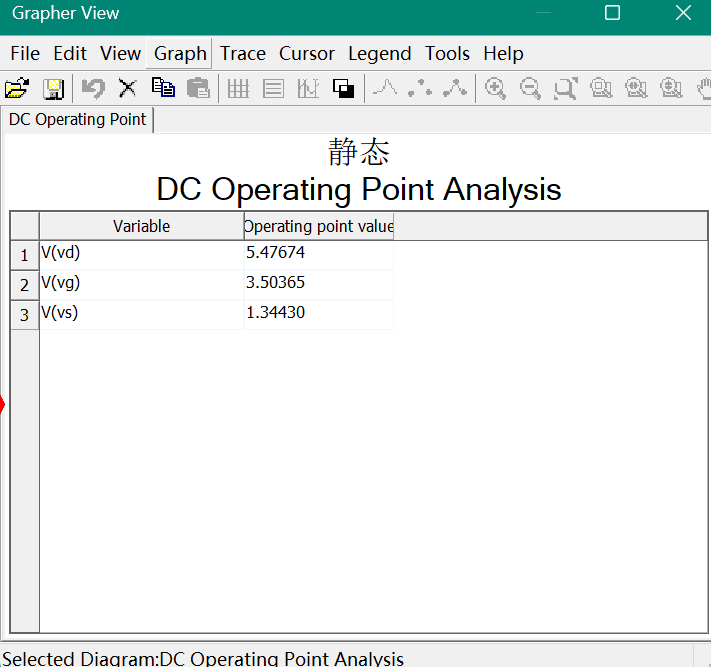
\includegraphics[width=0.5\textwidth]{2.3.png}
	\caption{直流工作点}
\end{figure}


\subsubsection{Single frequency ac analysis 得到输入输出电压曲线}
负载开路时电路图如下:
\begin{figure}[H]
	\centering
	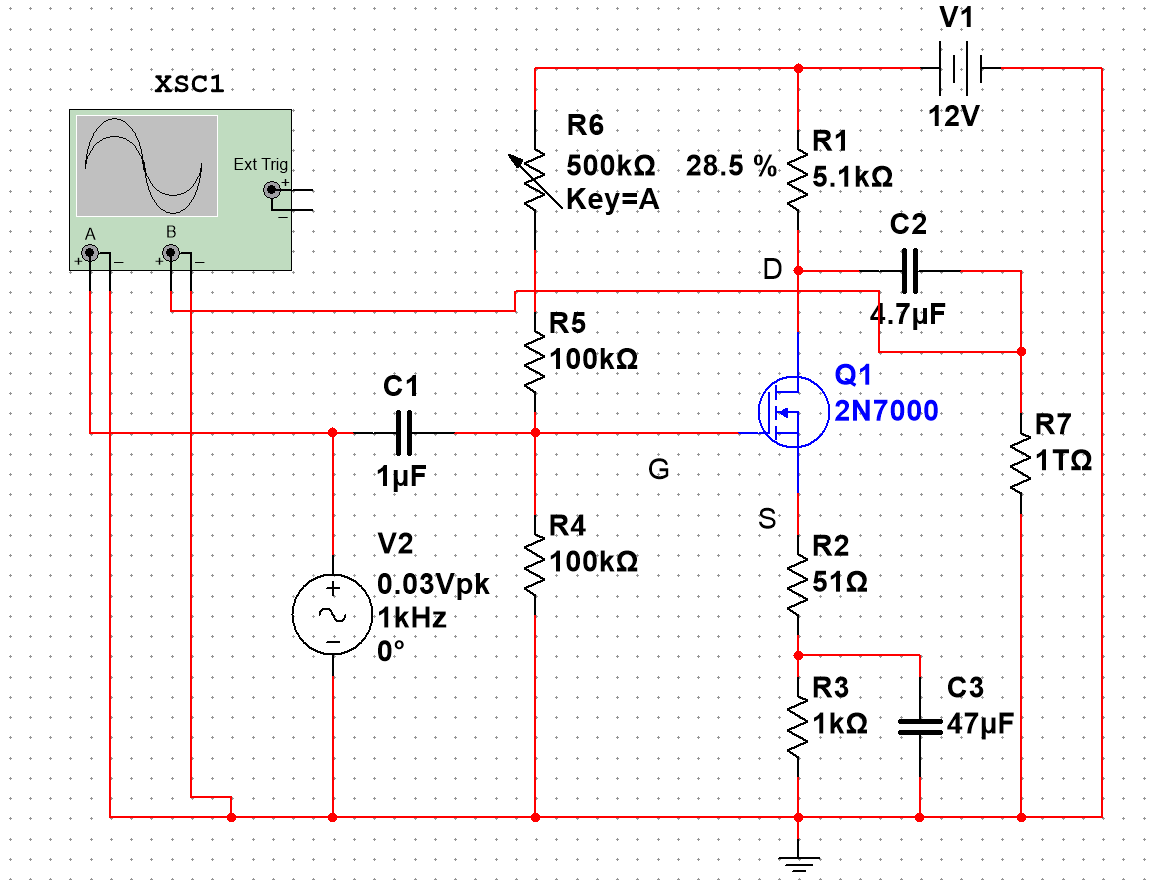
\includegraphics[width=0.7\textwidth]{2.4.png}	
	\caption{负载开路时电路图}
\end{figure}

\begin{itemize}
	\item 负载开路时(取 $R_7 = 1\text{T}\Omega$),通过观测示波器XSC1的输出,
	可以得到输出输入曲线,其中光标标记了输入输出的幅值,可以计算得到放大倍数约为
	$-\frac{1.332\text{V}}{29.872\text{mV}} \approx -44.59$。
	\item 负载为5.1 $\text{k}\Omega$ 时,通过观测示波器XSC1的输出,可以得到输出输入
	曲线,其中光标标记了输入输出的幅值,可以计算得到放大倍数约为
	$-\frac{668.076\text{mV}}{29.872\text{mV}} \approx -22.36$。
\end{itemize}

\begin{figure}[H]
	\subfigure[负载开路时波形]{
		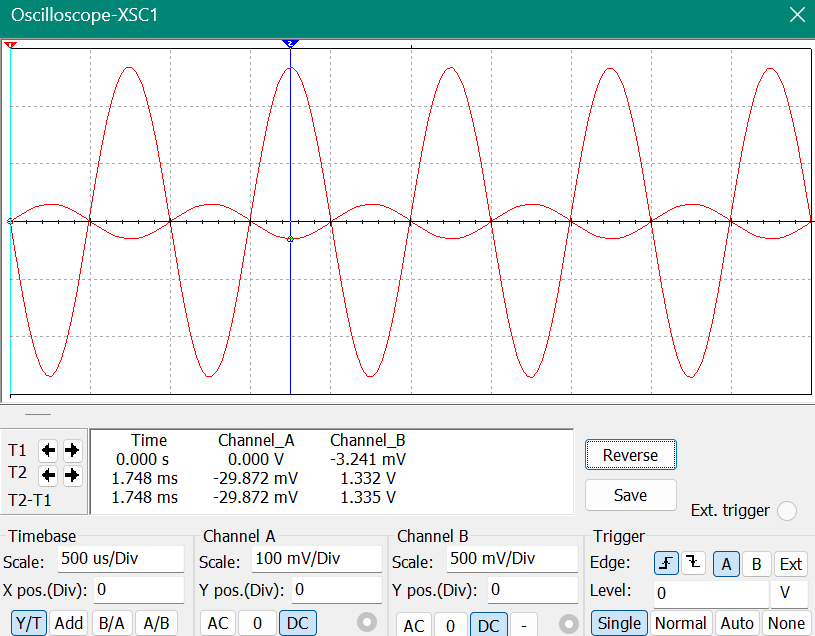
\includegraphics[width=0.48\textwidth]{2.5.png}
	}
	\subfigure[负载为5.1 $\text{k}\Omega$波形]{
		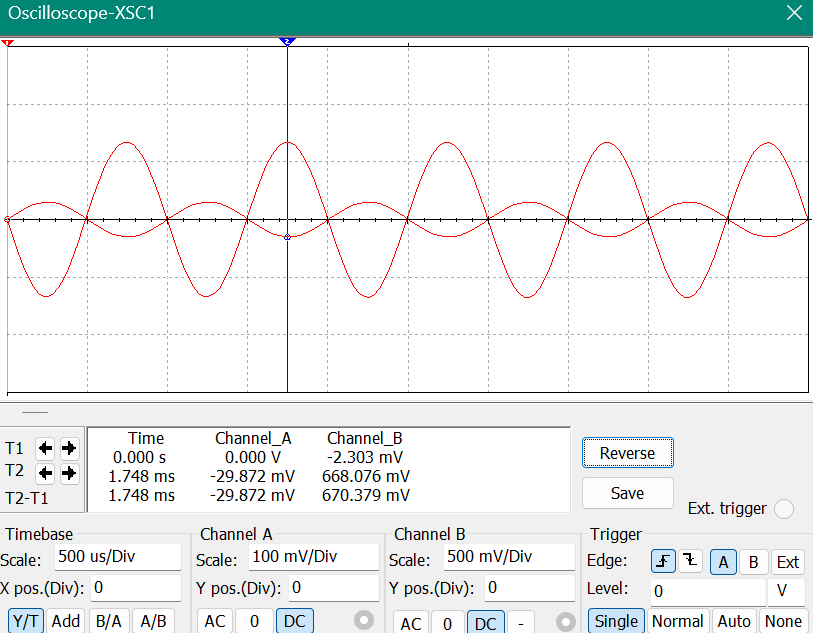
\includegraphics[width=0.48\textwidth]{2.6.png}
	}
\end{figure}

\subsubsection{AC Analysis 得到幅频特性曲线}
在分析中选择交流分析,得到负载开路时的幅频特性曲线:
\begin{figure}[H]
	\centering
	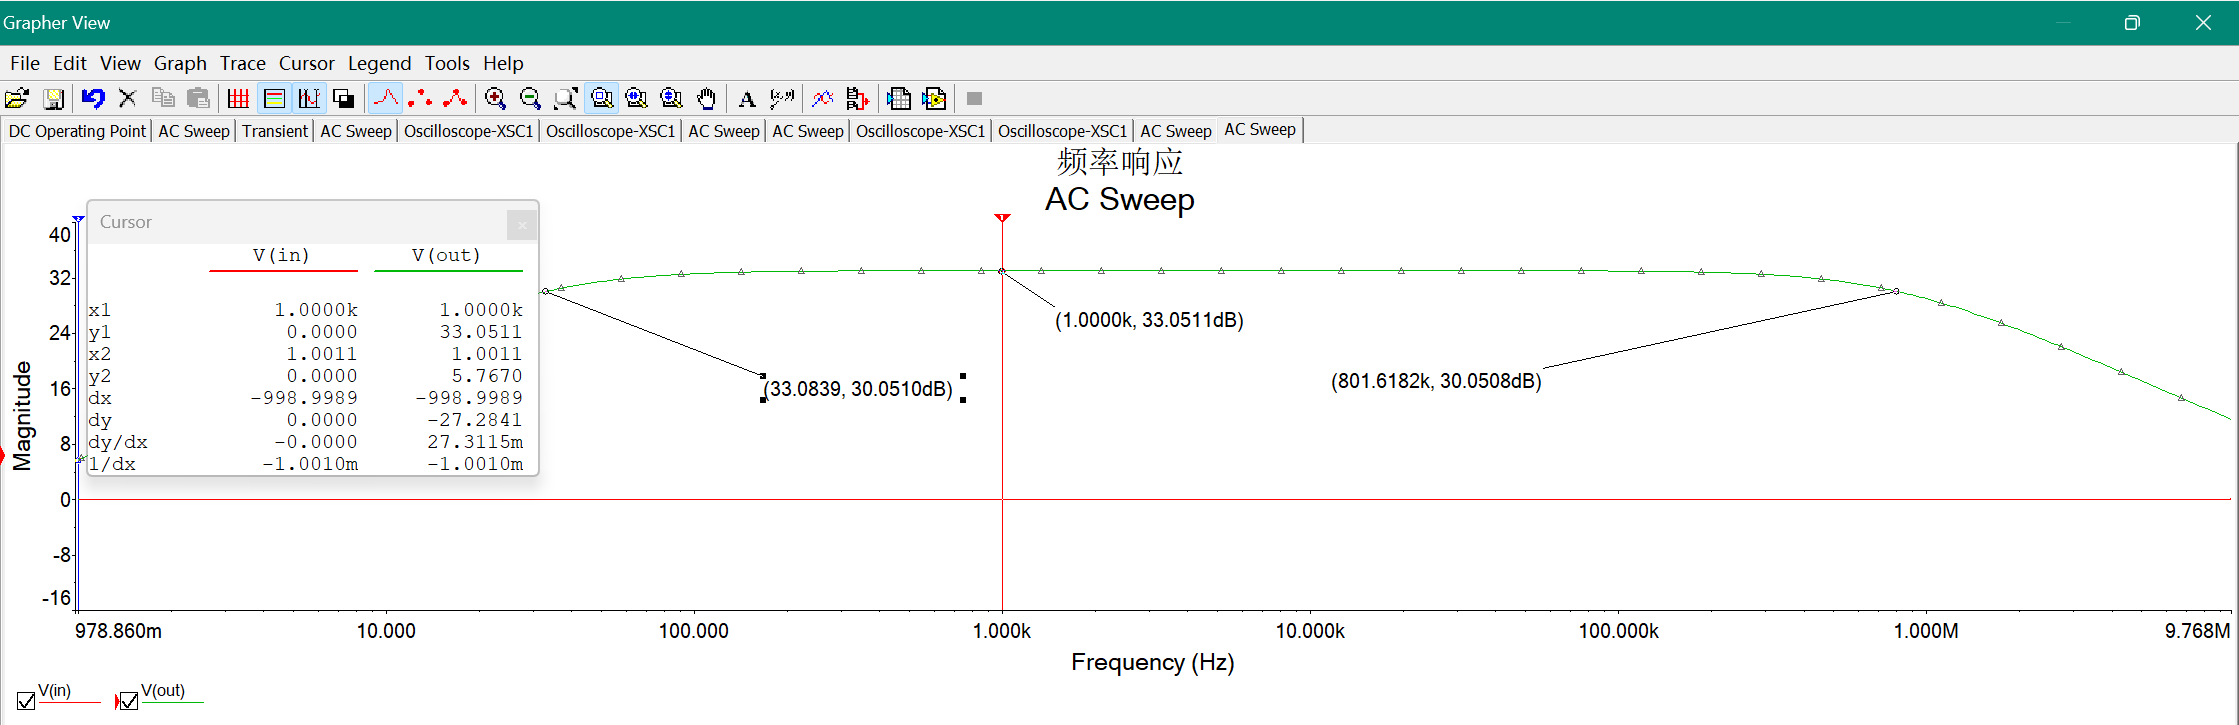
\includegraphics[width=0.8\textwidth]{2.7.png}	
	\caption{负载开路时幅频特性曲线}
\end{figure}

设置输入信号频率为1kHZ时,得到通频带增益为33.0511dB左右。
上图光标标记了通带增益以及-3dB处的上下限频率。可以得到
上下限频率:$f_L=33.0839$Hz,$f_H=801.6182$kHz。

\subsubsection{AC 模式测量输入阻抗}
在分析中选择交流分析,可以得到输入电阻-频率曲线:

\begin{figure}[H]
	\centering
	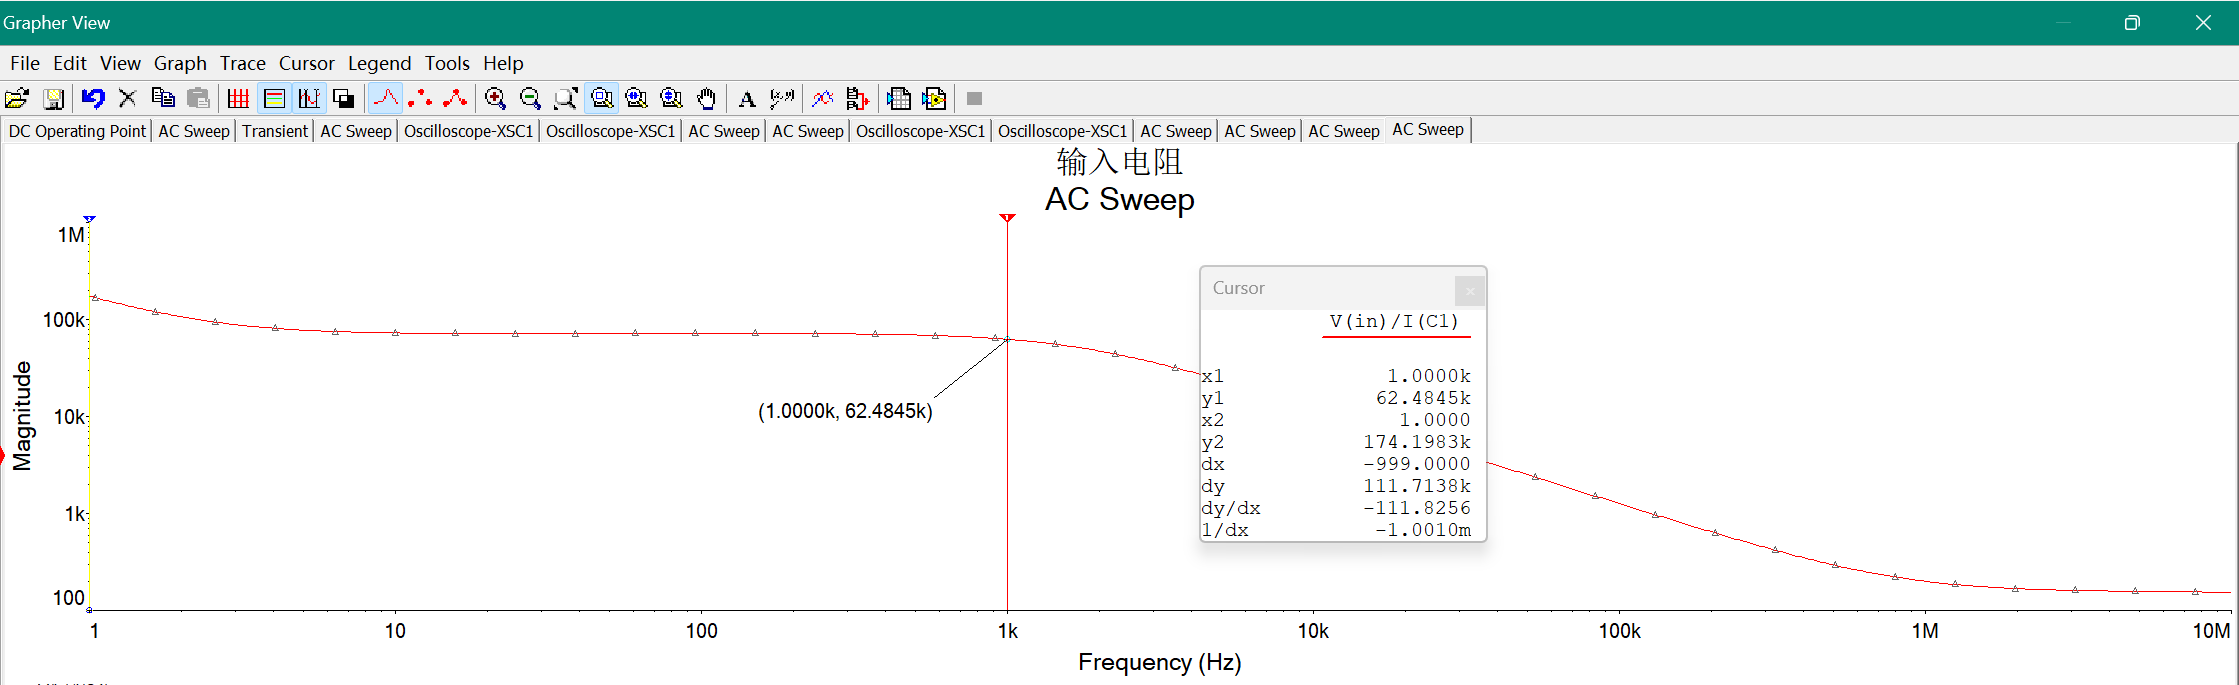
\includegraphics[width=0.8\textwidth]{2.8.png}	
	\caption{输入电阻-频率曲线}
\end{figure}

根据光标可以观察到$R_i=62.4845\mathrm{k\Omega}$

\subsubsection{AC 模式测量输出阻抗}
输出电阻的测量略有不同,需要调整为在输入短路的条件下计算$v_o/v_i$,修改的电路图如下:

\begin{figure}[H]
	\centering
	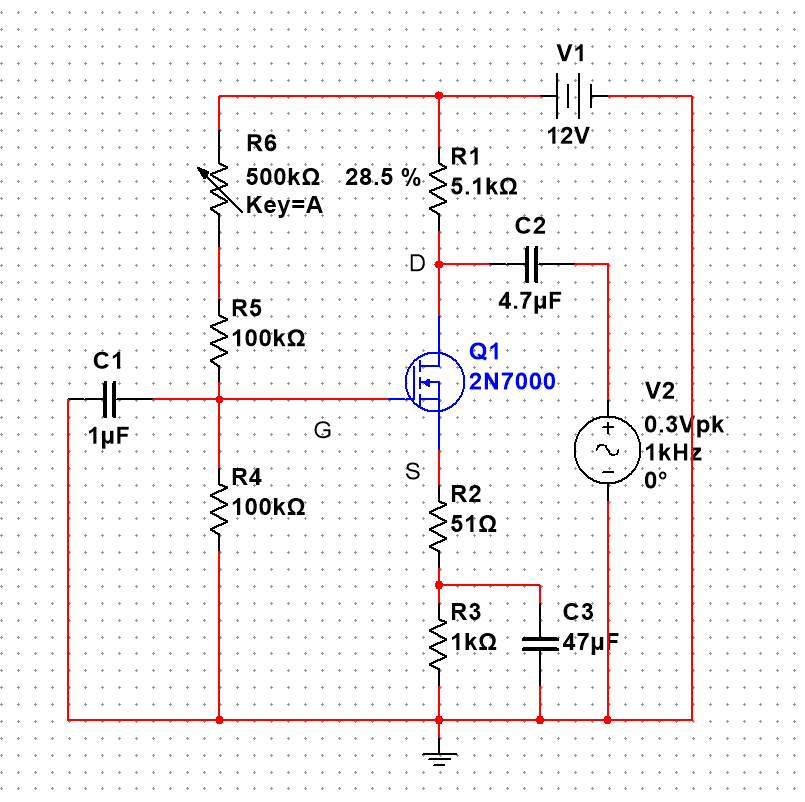
\includegraphics[width=0.7\textwidth]{2.9.png}	
	\caption{输出电阻测量电路图}
\end{figure}

输出电阻-频率曲线如下:

\begin{figure}[H]
	\centering
	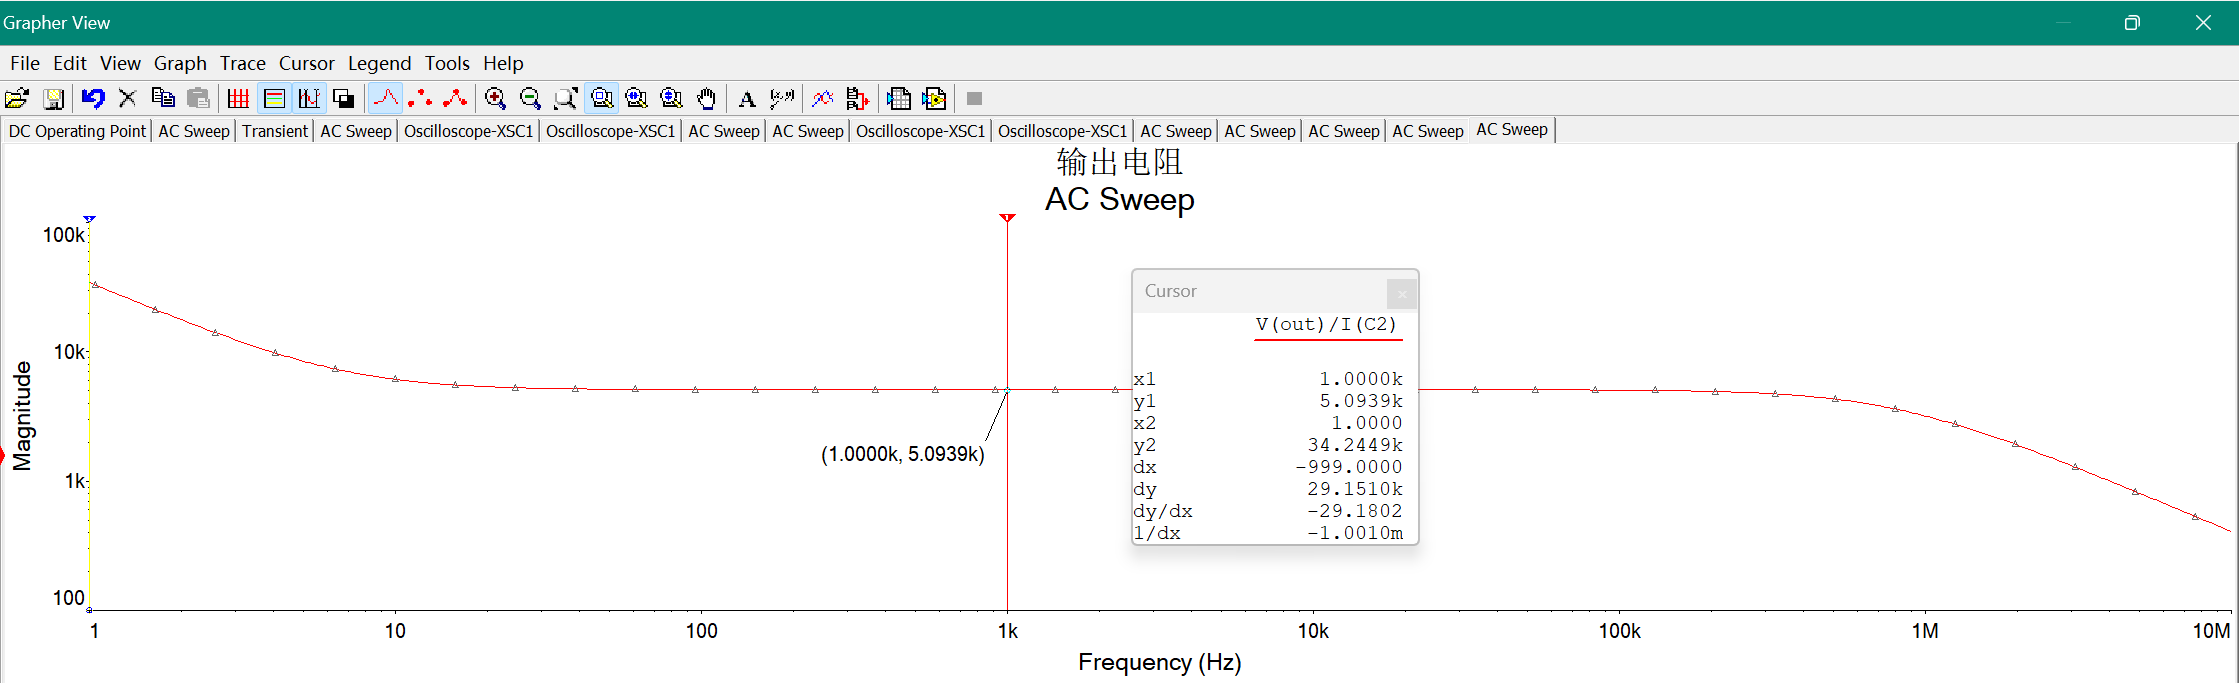
\includegraphics[width=0.8\textwidth]{2.10.png}	
	\caption{输出电阻-频率曲线}
\end{figure}

根据光标可以观察到$R_o=5.0939\mathrm{k\Omega}$

\subsubsection{观察失真波形}
分别设置电位器位于满阻值的25$\%$和82$\%$,在分析中选择瞬态分析,得到饱和失真波形和截止失真波形:

\begin{figure}[H]
	\subfigure[饱和失真波形]{
		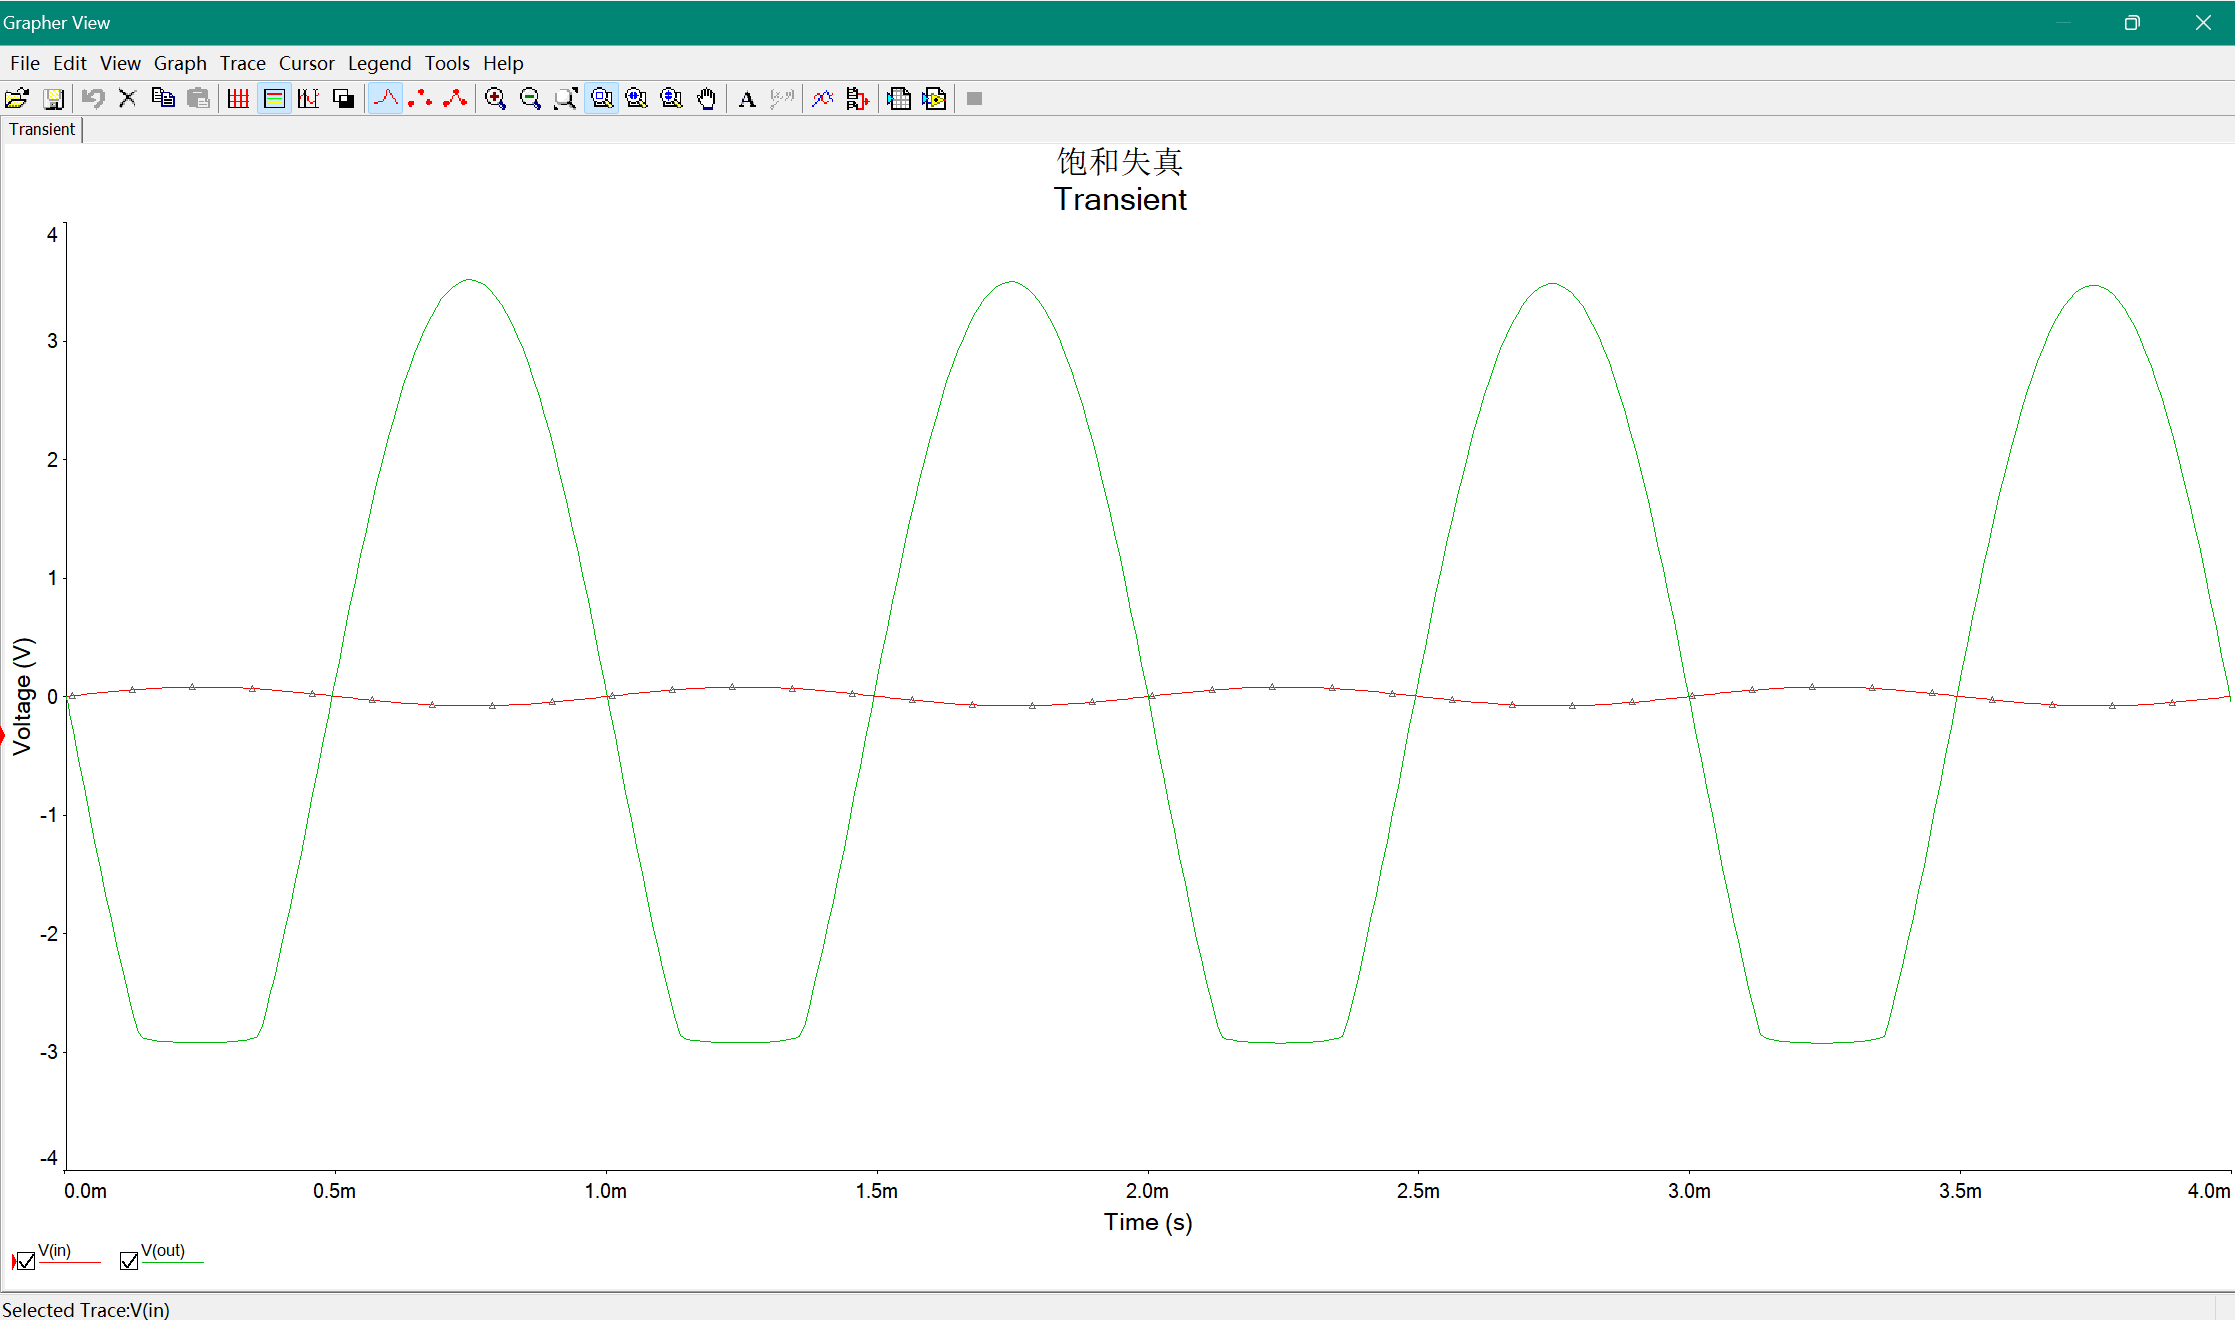
\includegraphics[width=0.48\textwidth]{2.11.png}
	}
	\subfigure[截止失真波形]{
		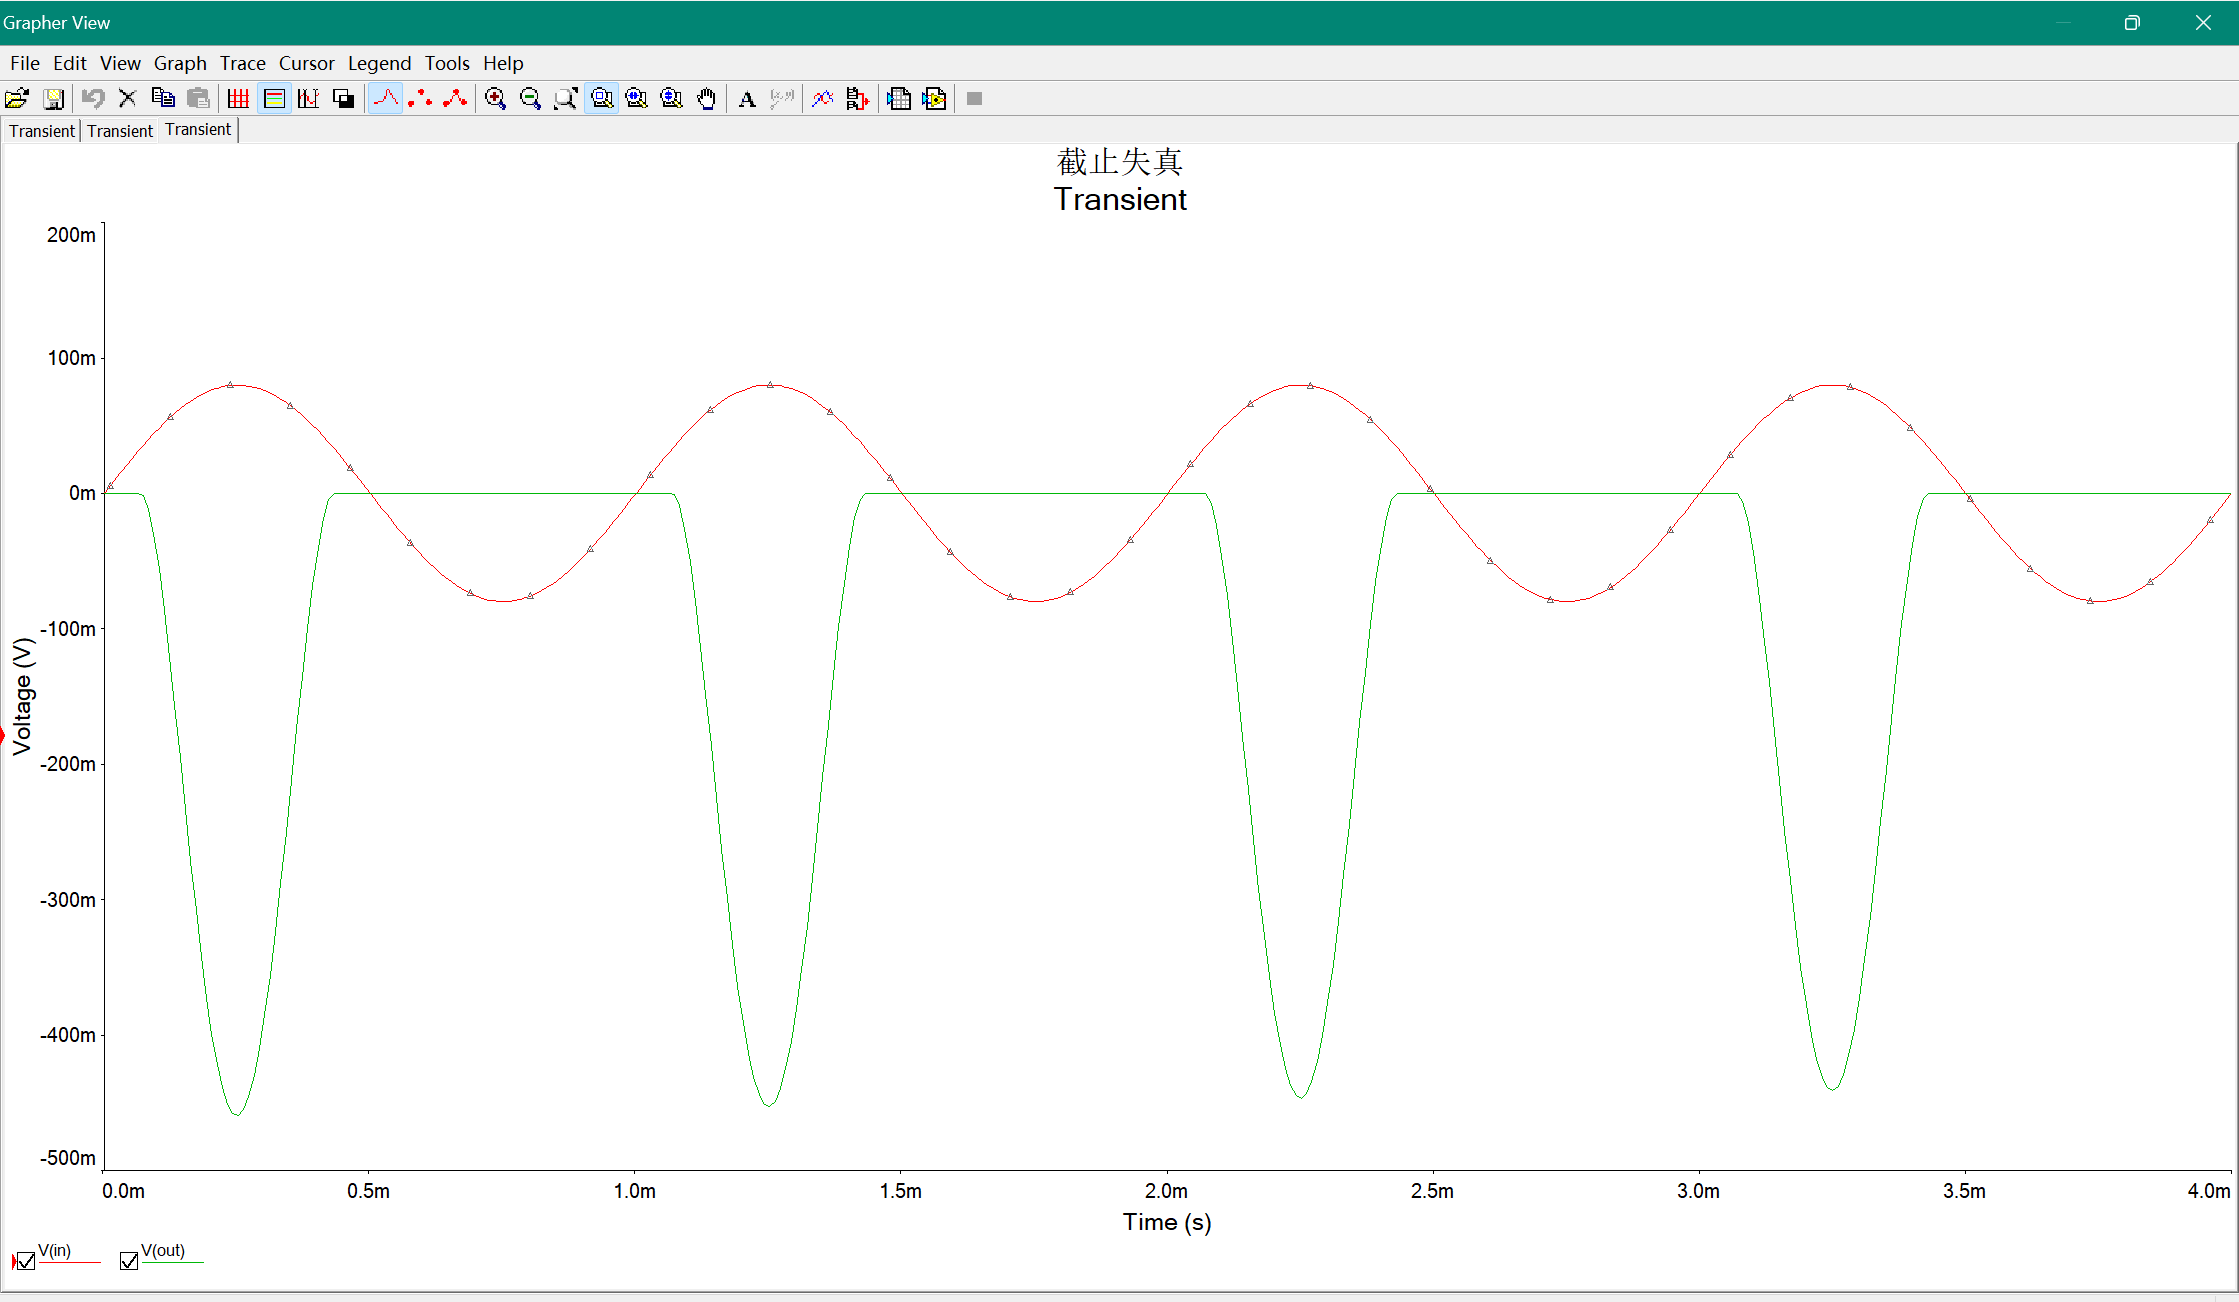
\includegraphics[width=0.48\textwidth]{2.12.png}
	}
\end{figure}

\subsubsection{MOSFET输出特性曲线仿真}
电路图如下:

\begin{figure}[H]
	\centering
	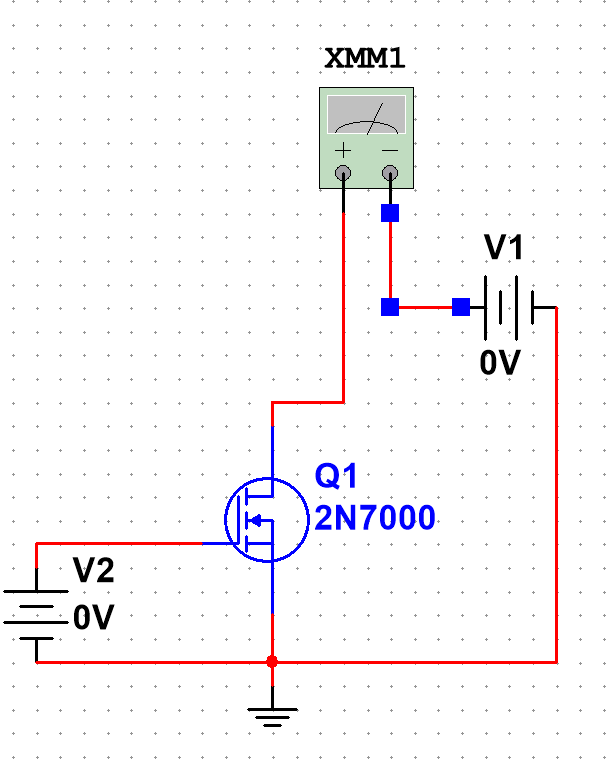
\includegraphics[width=0.6\textwidth]{2.13.png}	
	\caption{MOSFET输出特性曲线仿真电路图}
\end{figure}

在分析中选择直流扫描分析,扫描变量为 $V_1(V_{DS})$,由0$\text{V}$开始至8$\text{V}$结束,增量为0.01$\text{V}$。
对于扫描变量$V_2(V_{GS})$,由1.9$\text{V}$开始至2.3$\text{V}$结束,增量为0.05$\text{V}$。
得到输出特性曲线如下:

\begin{figure}
	\centering
	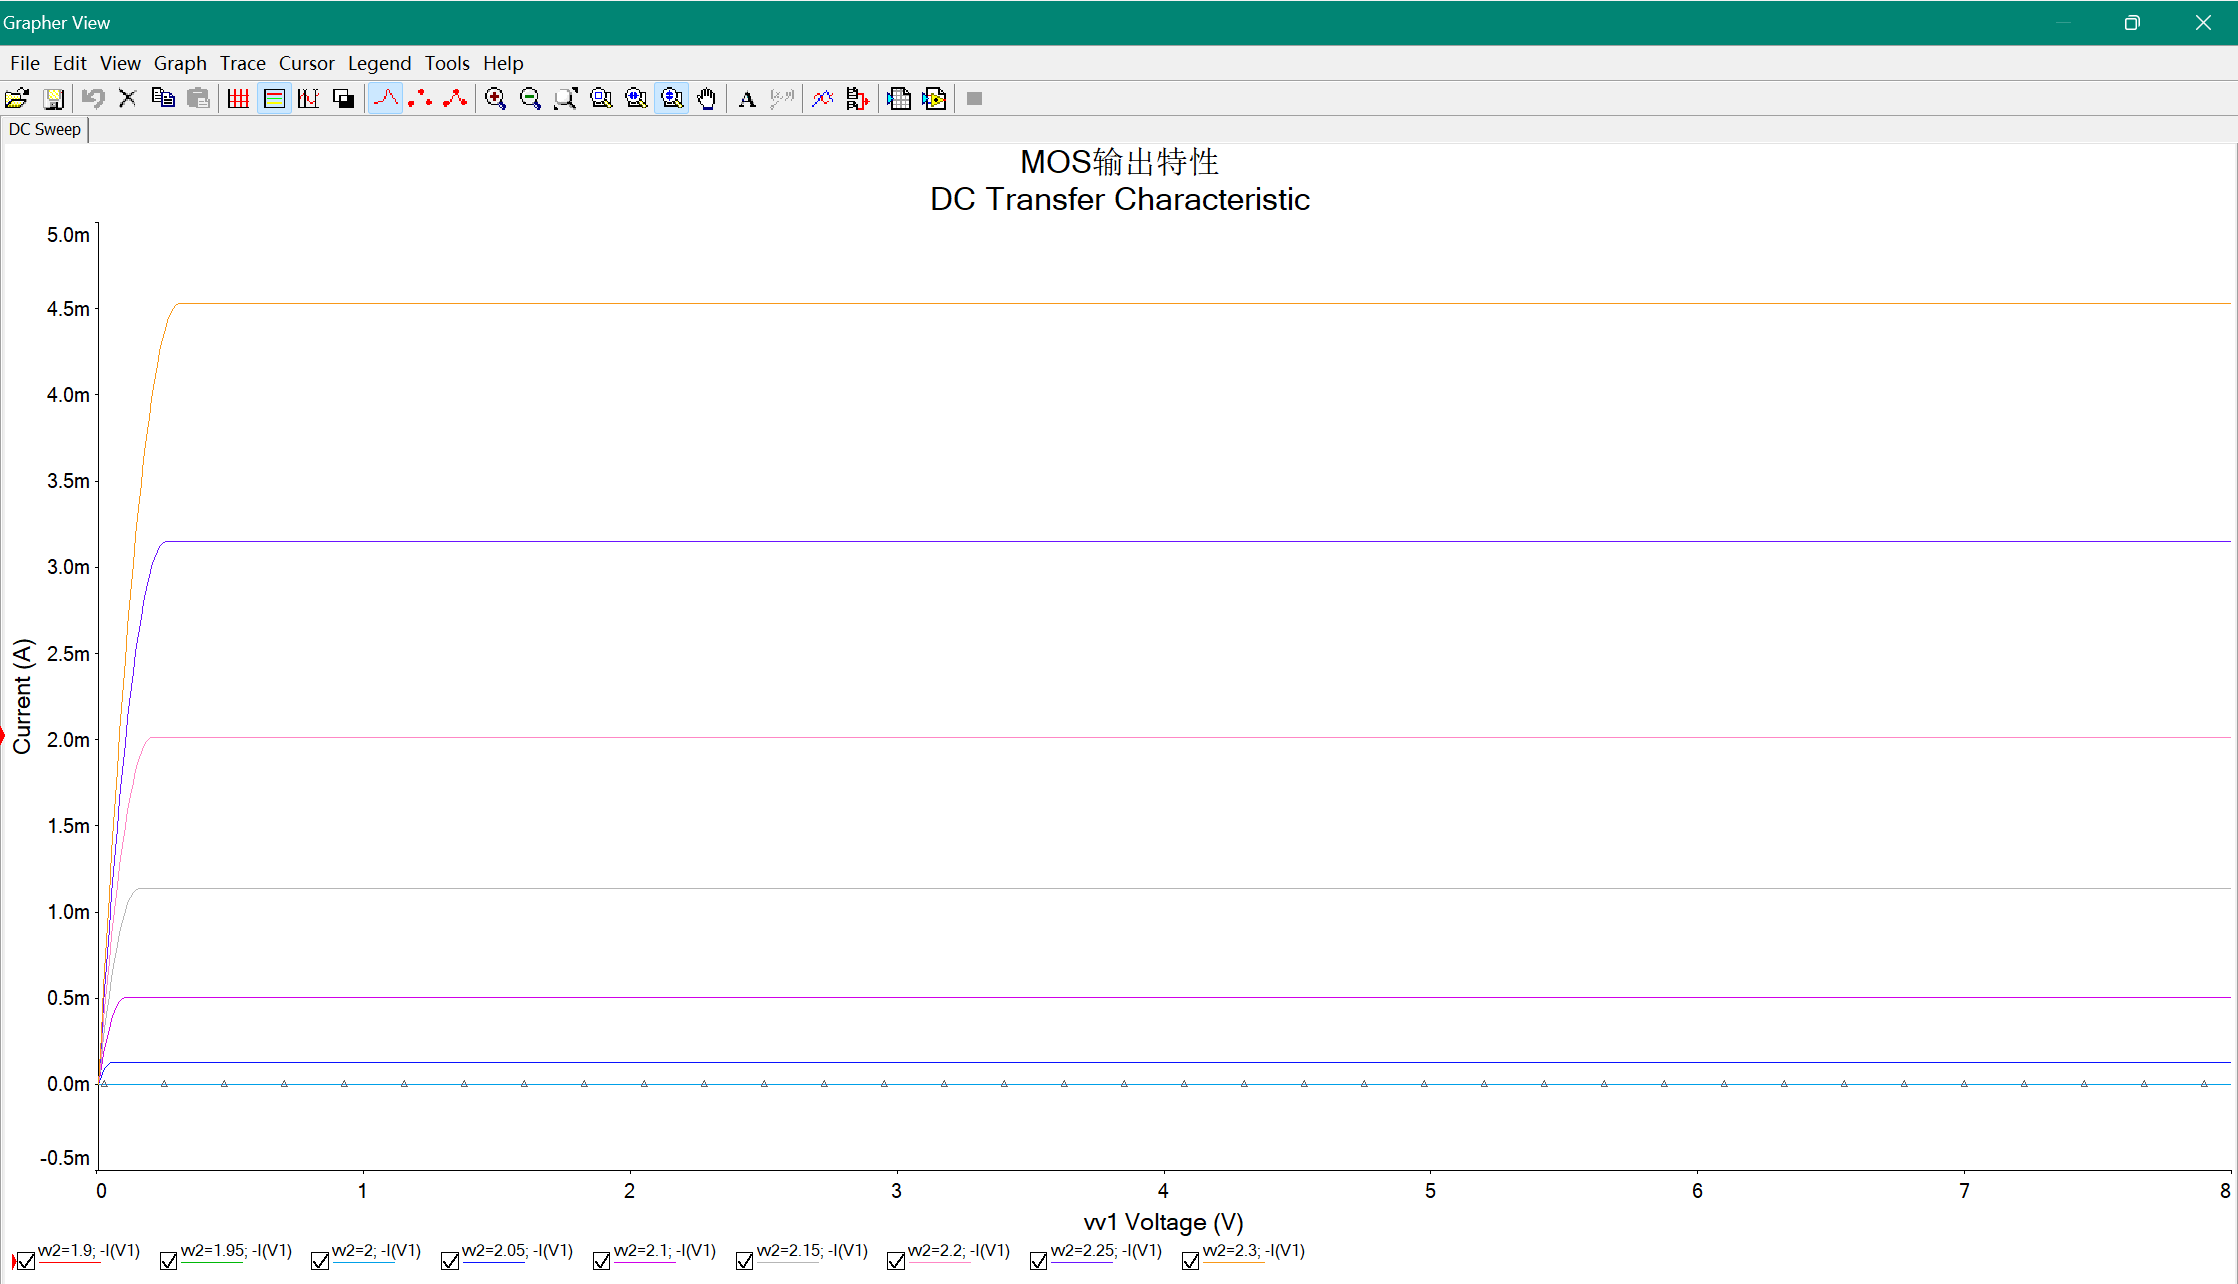
\includegraphics[width=0.8\textwidth]{2.14.png}
	\caption{MOSFET输出特性曲线}
\end{figure}

\subsubsection{MOSFET转移特性曲线仿真}
电路图如下:

\begin{figure}[H]
	\centering
	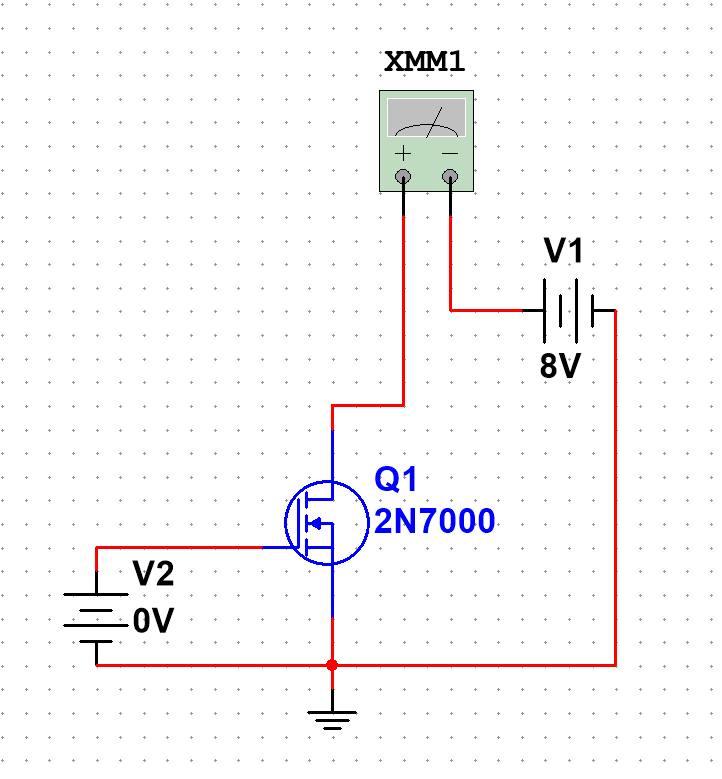
\includegraphics[width=0.5\textwidth]{2.15.png}	
	\caption{MOSFET转移特性曲线仿真电路图}
\end{figure}

在分析中选择直流扫描分析,设置 $V_{2} = 8V$,扫描变量为$V_2(V_{GS})$,由0$V$开始至8$V$结束,
增量为0.01$V$,得到转移特性曲线如下:

\begin{figure}
	\centering
	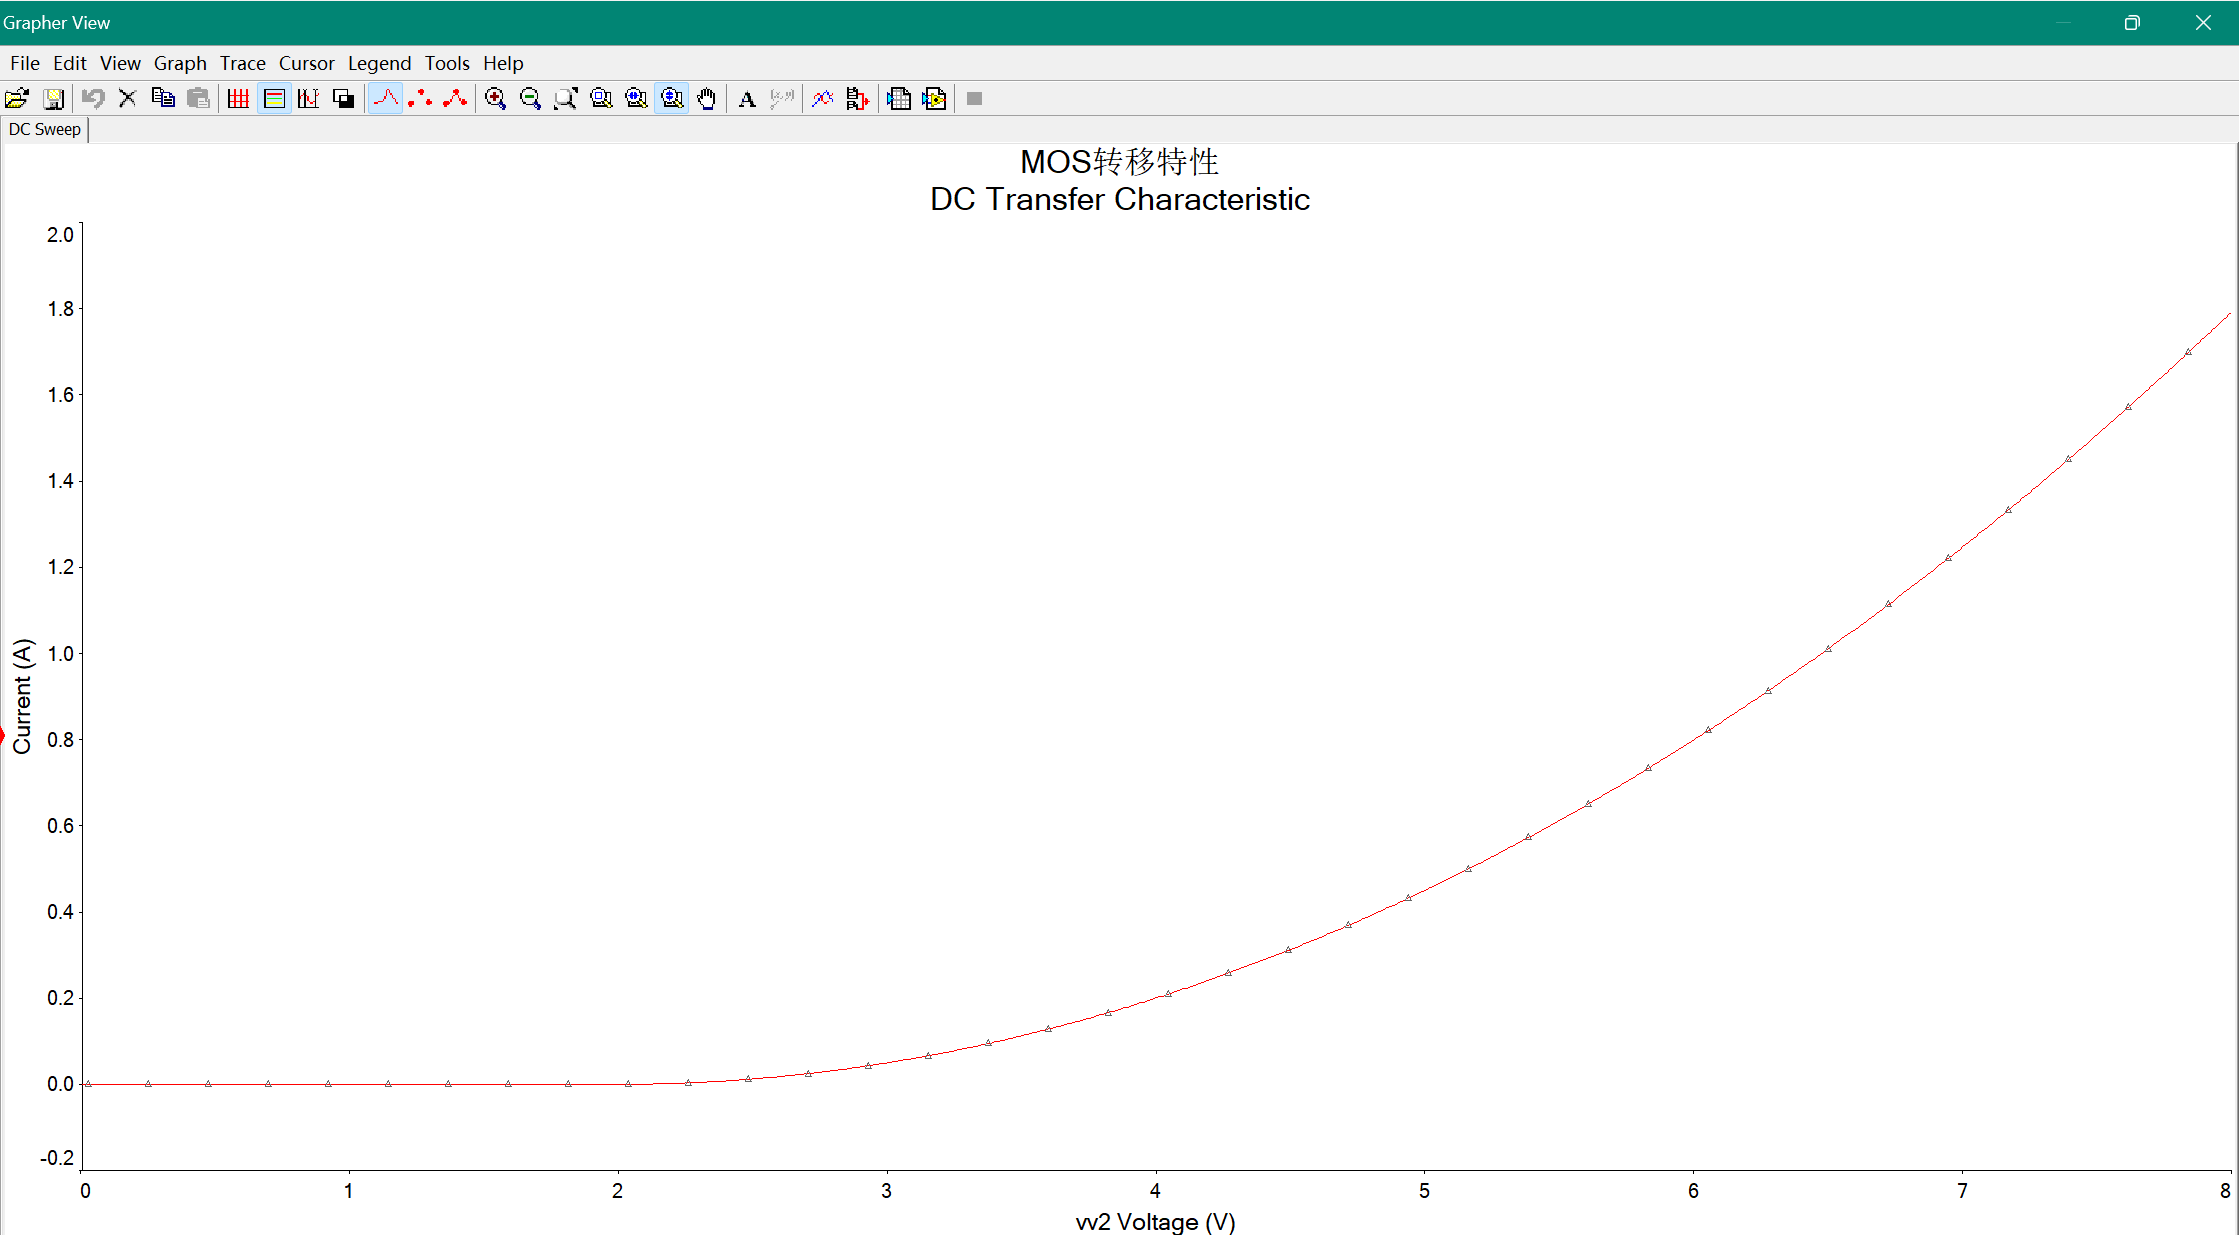
\includegraphics[width=0.6\textwidth]{2.16.png}
	\caption{MOSFET转移特性曲线}
\end{figure}

\subsection{单极 MOSFET 共源放大电路插板实验}

\subsubsection{测试静态工作点}
实验中数据记录表格如下:

\begin{table}[H]
	\centering
	\begin{tabular}{|c|c|c|c|c|c|}
	\hline
	\multicolumn{3}{|c|}{实测值} & \multicolumn{3}{c|}{计算值} \\
	\hline
	\( V_G/\mathrm{V} \) & \( V_S/\mathrm{V} \) & \( V_D/\mathrm{V} \) & \( I_{DQ} = \frac{V_S}{R_{ss}} \) (mA) & \( V_{GSQ} = V_G - V_S \) (V) & \( V_{DSQ} = V_D - V_S \) (V) \\
	\hline
	2.9371 & 1.2960 & 5.4839 & 1.268 & 1.641 & 4.1879 \\
	\hline
	\multicolumn{6}{|c|}{实测电阻值} \\
	\hline
	\multicolumn{6}{|c|}{\( R_{g1} = 98.424\mathrm{k\Omega} \) , \( R_{g2} = 98.635\mathrm{k\Omega}\) , \( R_d = 5.151\mathrm{k\Omega}\) , \( R_s = 1.022\mathrm{k\Omega}\)}\\
	\hline
	\end{tabular}
\end{table}

\subsubsection{测试放大电路的输入、输出波形和通带电压增益}
负载开路时和负载为 5.1$\text{k}\Omega$ 时的输入、输出波形分别如下:

\begin{figure}[H]
	\subfigure[负载开路时波形]{
		\centering
		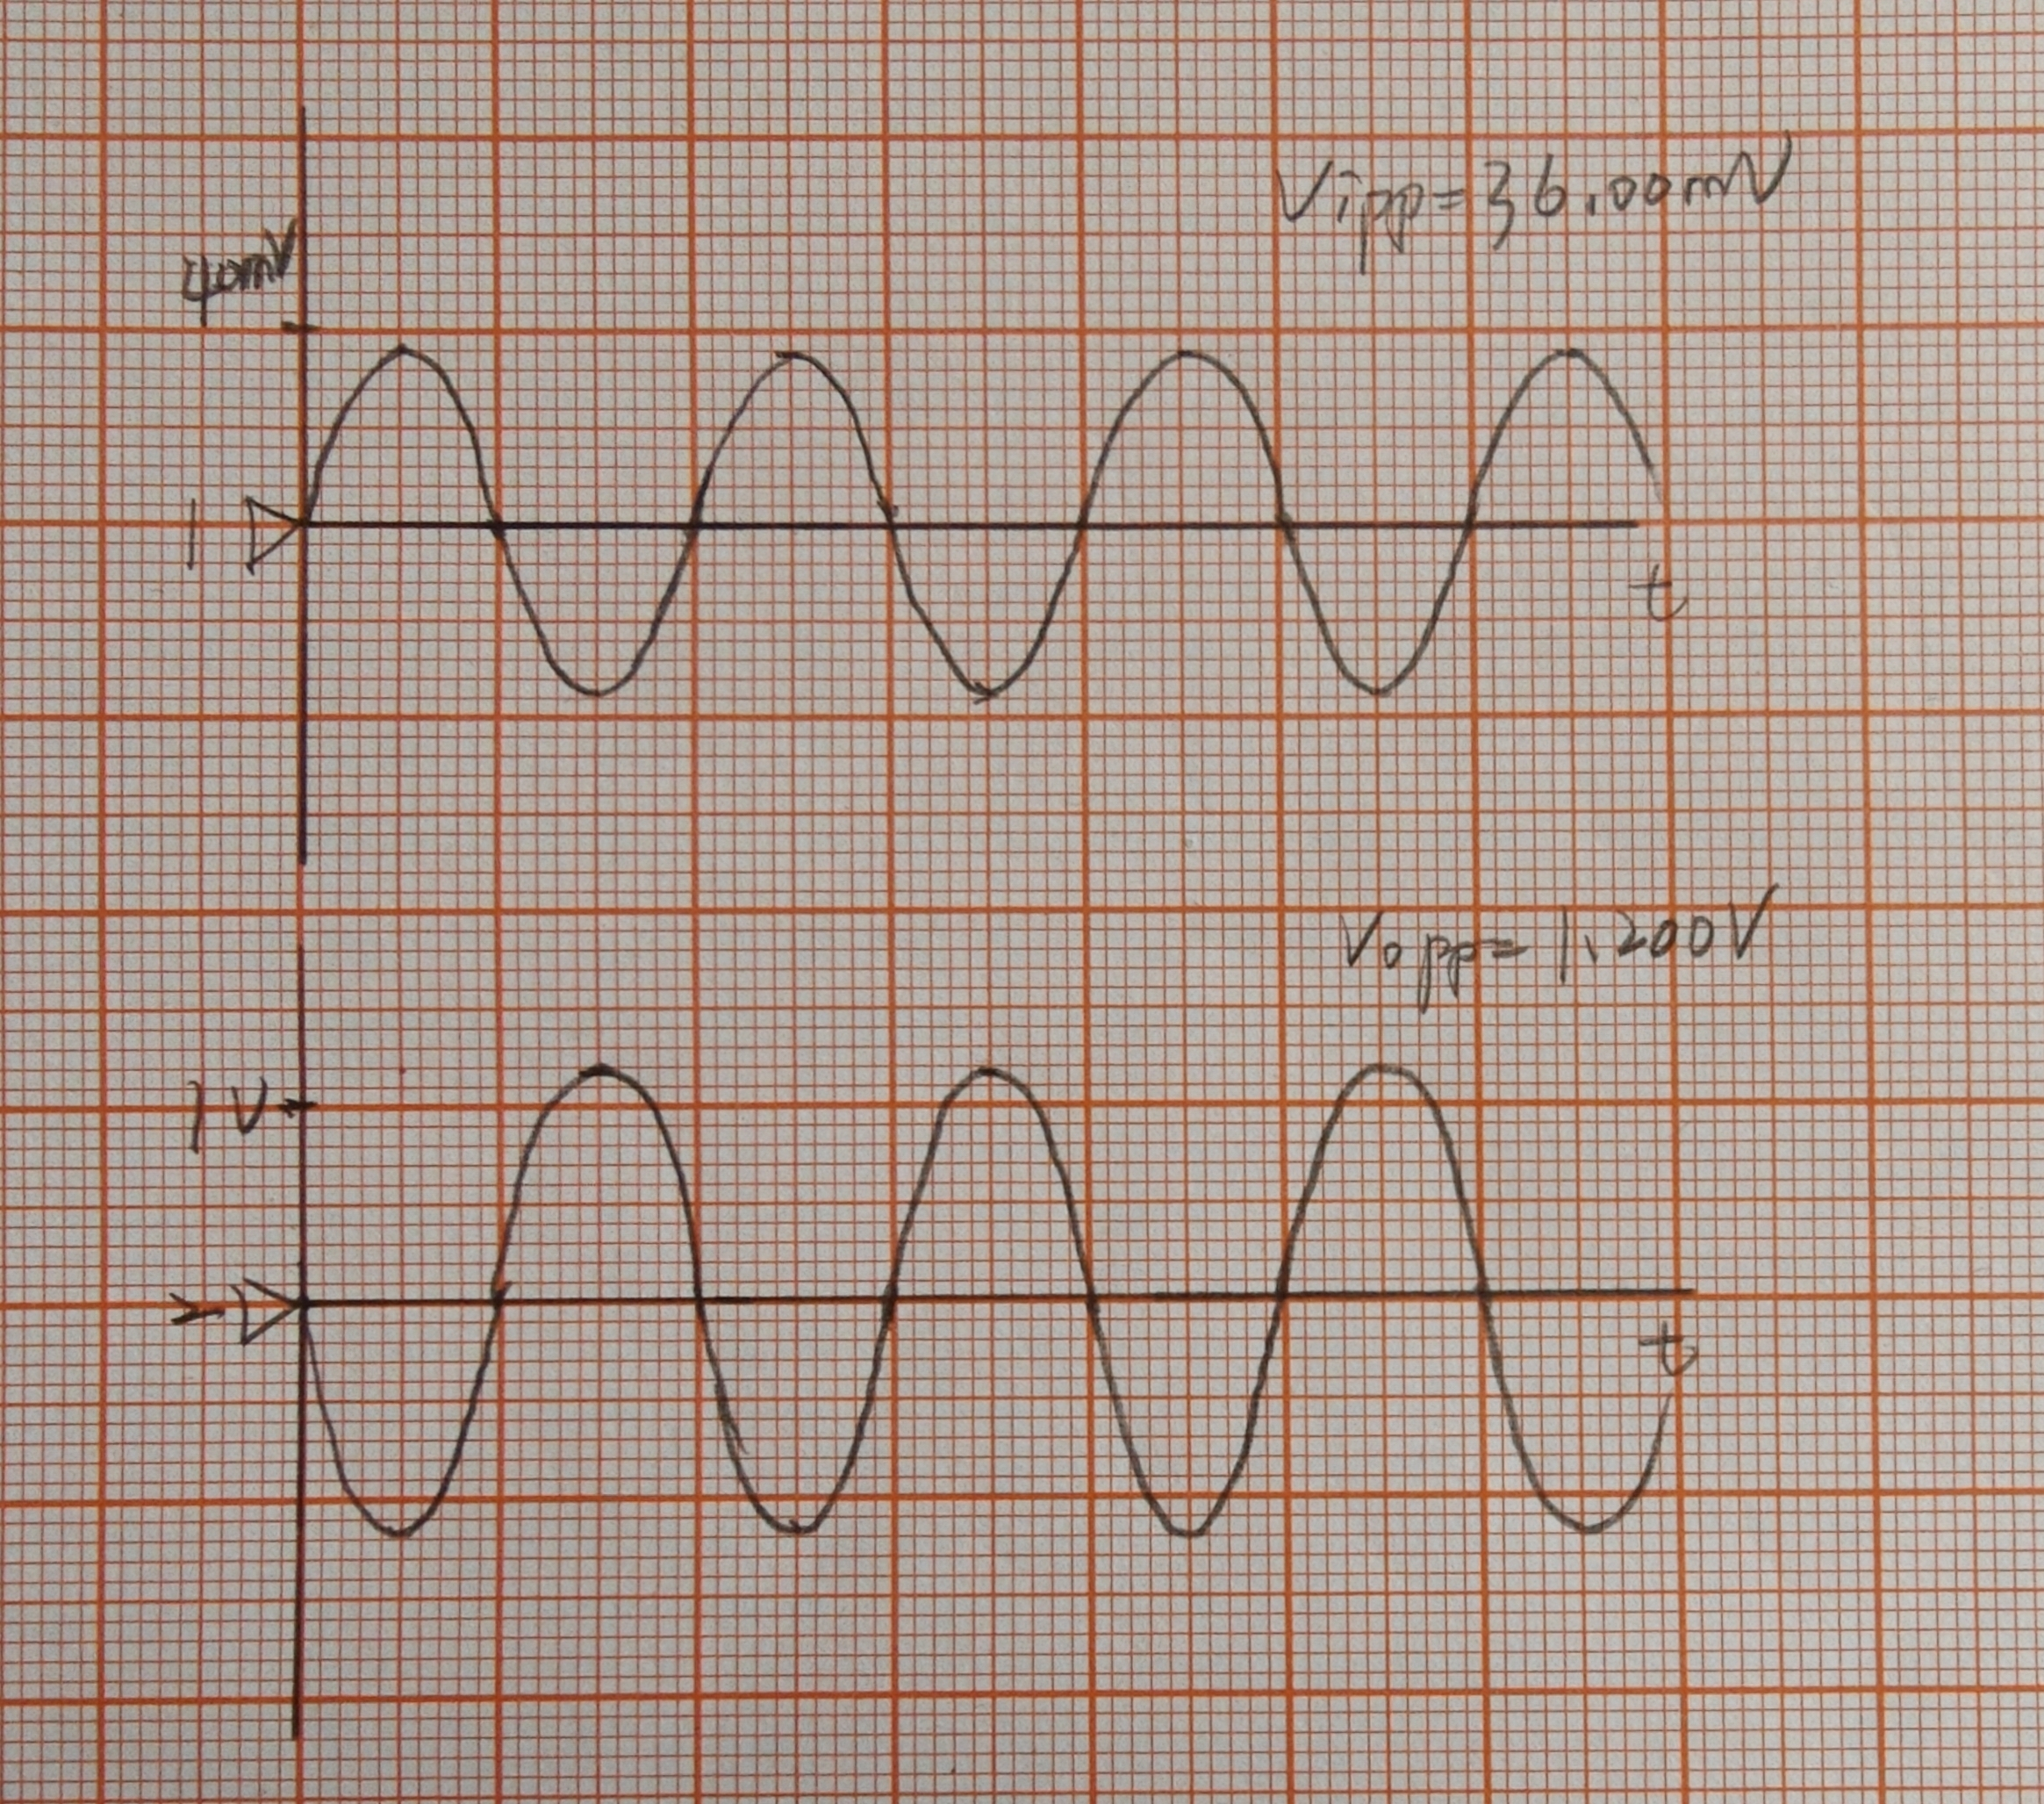
\includegraphics[width=0.48\textwidth]{2.17.jpg}
	}
	\subfigure[负载为$R_L$时波形]{
		\centering
		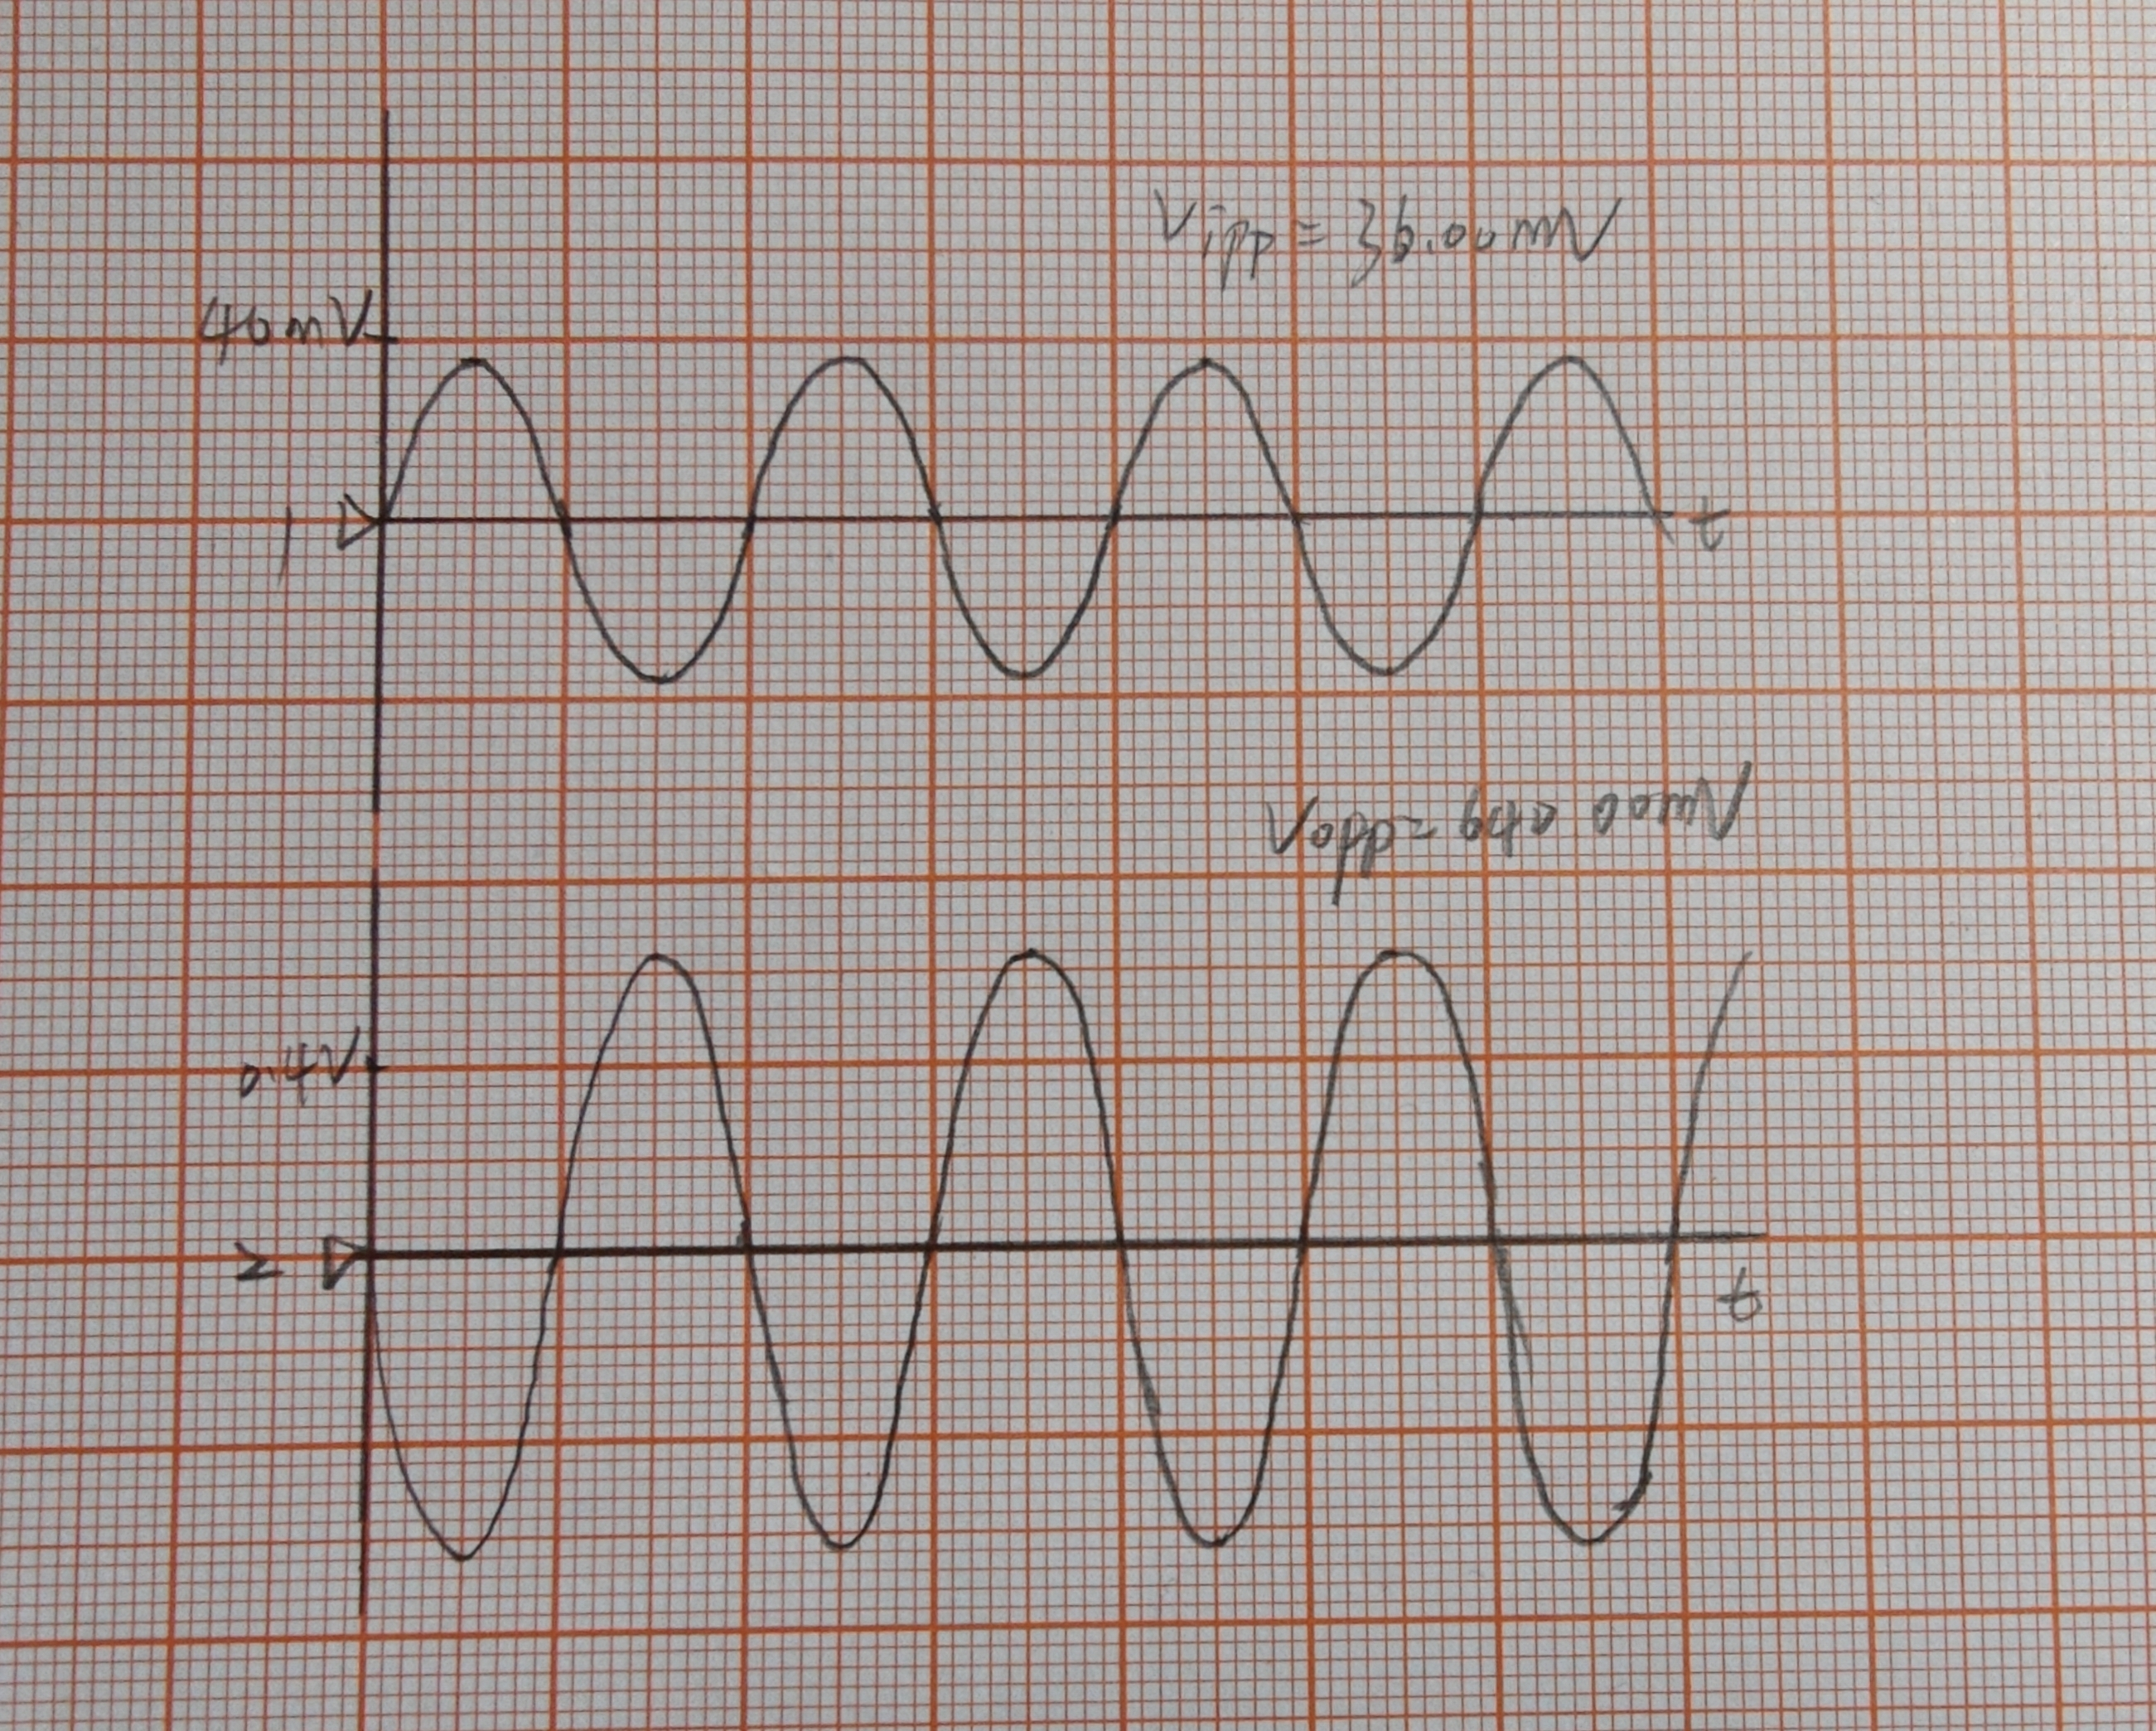
\includegraphics[width=0.48\textwidth]{2.18.jpg}
	}
\end{figure}

实验数据记录表格如下:

\begin{table}[H]
	\centering
	\begin{tabular}{|c|c|c|c|c|c|}
			\hline
			\shortstack{负载\\情况} & \shortstack{$v_i$峰-峰\\值$V_{ipp}$/mV} & 
			\shortstack{$v_o$峰-峰值\\$V_{opp}$/mV} & 
			\shortstack{$|A_v|=$\\$V_{opp}/V_{ipp}$} & 
			\shortstack{$|A_v|$的\\理论值} & 
			\shortstack{相对\\误差}\\
			\hline
			负载开路 & 36 & 1200 & 33.33 & 28.87 & 15.45\%\\
			\hline
			$R_L=5.1\mathrm{k\Omega}$ & 36 & 640 & 17.78 & 14.58 & 21.95\%\\
			\hline		
		\end{tabular}
\end{table}

\subsubsection{测试放大电路的输入电阻}
测量得到此时的$R=55.87\mathrm{k\Omega}$。开关S闭合时,$V_{opp1} = 1.16\mathrm{V}$
开关S断开时,输出信号的峰峰值 $V_{opp2} = 0.7\mathrm{V}$,则输入电阻为:

$$
R_{i} = \frac{V_{opp2}}{V_{opp1}-V_{opp2}} \cdot R = 77.77\mathrm{k\Omega}
$$

\subsubsection{测试放大电路的输出电阻}
测量得到此时的$R_L=5.151\mathrm{k\Omega}$,由前面测得的负载开路时的输出电压 $v_{o}$ 
和接入$R_L$时的输出电压$v_{o}^{'}$可计算输出电阻:
$$
R_{o} = \frac{v_{o}^{'}-v_o}{v_o} \cdot R_L = 4.51 \mathrm{k\Omega}
$$

\subsubsection{测试放大电路的通频带}
下表记录了通频带的测量数据:

\begin{table}
	\centering
	\begin{tabular}{|c|c|c|c|c|c|c|c|c|c|c|}
		\hline
		输入信号频率 $f/\mathrm{Hz}$ & 25 & 30 & 60 & 100 & 500k & 700k & 850k & 900k & 1M & 1.25M \\
		\hline
		$V_{opp}/\mathrm{V}$ & 0.820 & 0.900 & 1.06 & 1.14 & 1.12 & 1.04 & 0.980 & 0.960 & 0.920 & 0.820 \\
		\hline
	\end{tabular}
\end{table}

由于负载开路时输出波形的峰峰值为$1.16\mathrm{V}$,降到0.707倍时为
$1.16 \times 0.707 = 0.820\mathrm{V}$,则可以得到上下限频率:$f_L = 25$ Hz,$f_H = 1.25$MHz

\subsubsection{观察失真波形}
下图定性绘制了饱和失真和截止失真的波形:

\begin{figure}[H]
	\subfigure[饱和失真波形]{
		\centering
		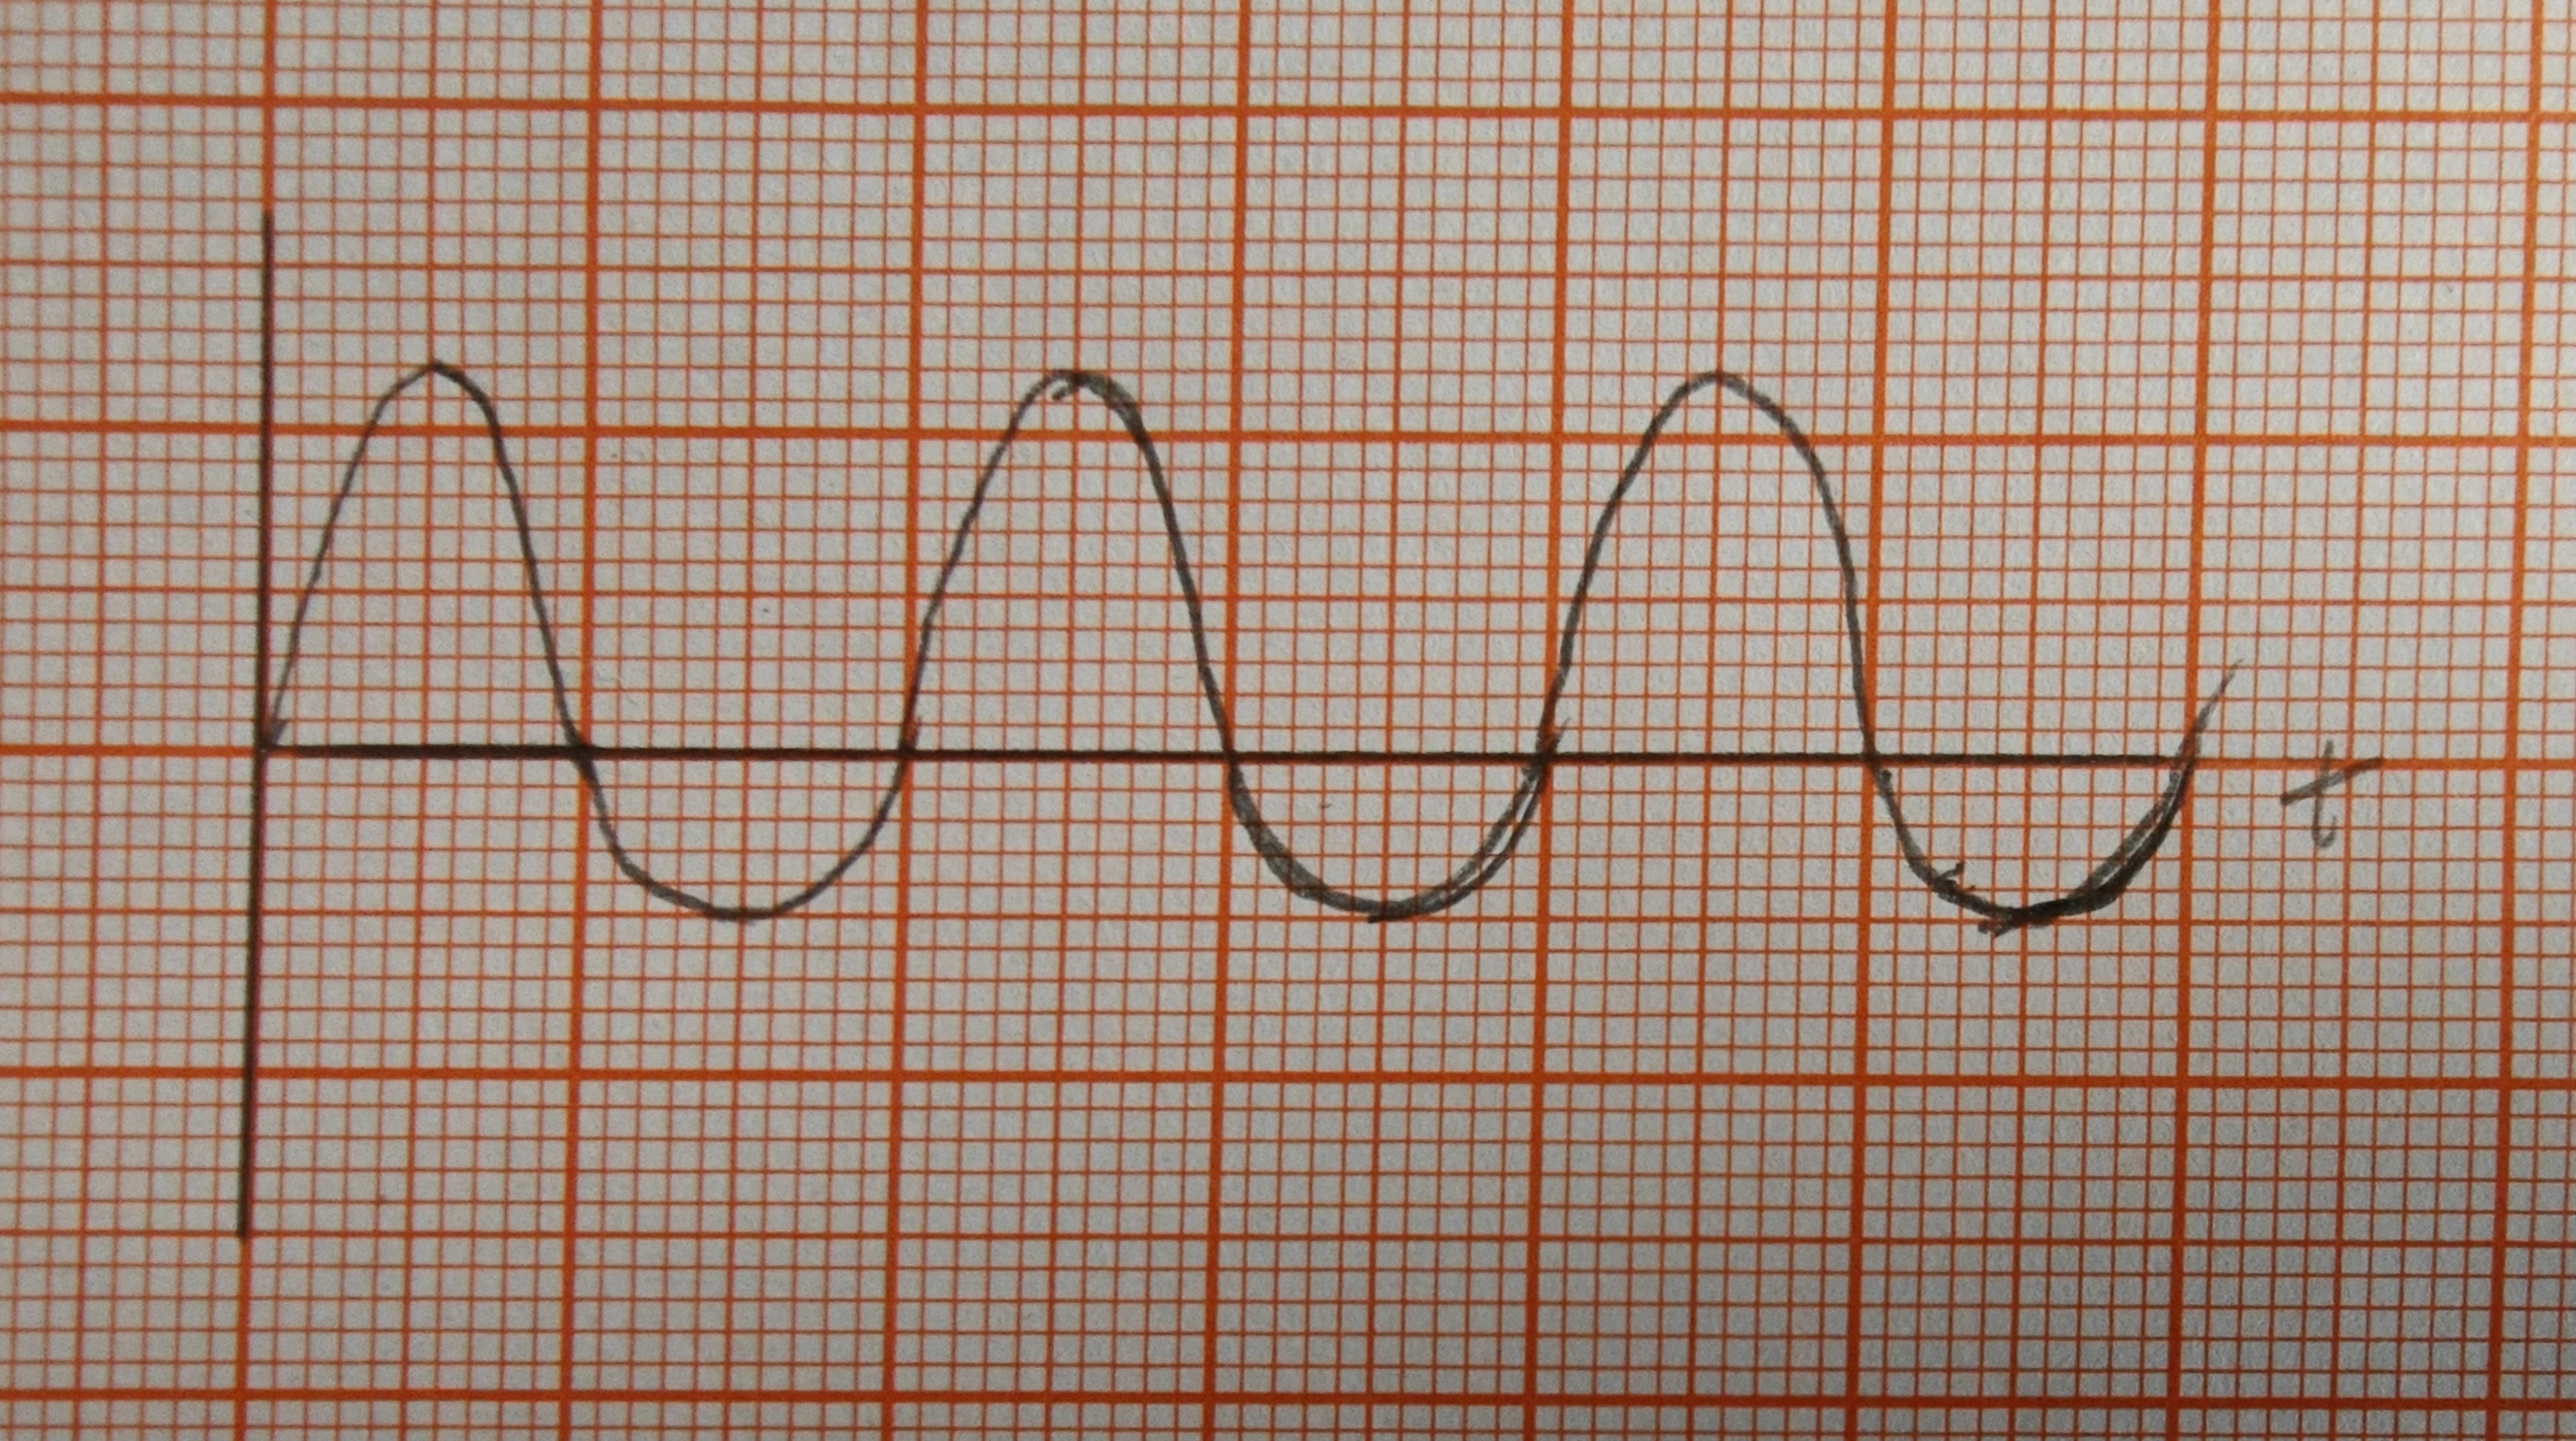
\includegraphics[width=0.48\textwidth]{2.19.jpg}
	}
	\subfigure[截止失真波形]{
		\centering
		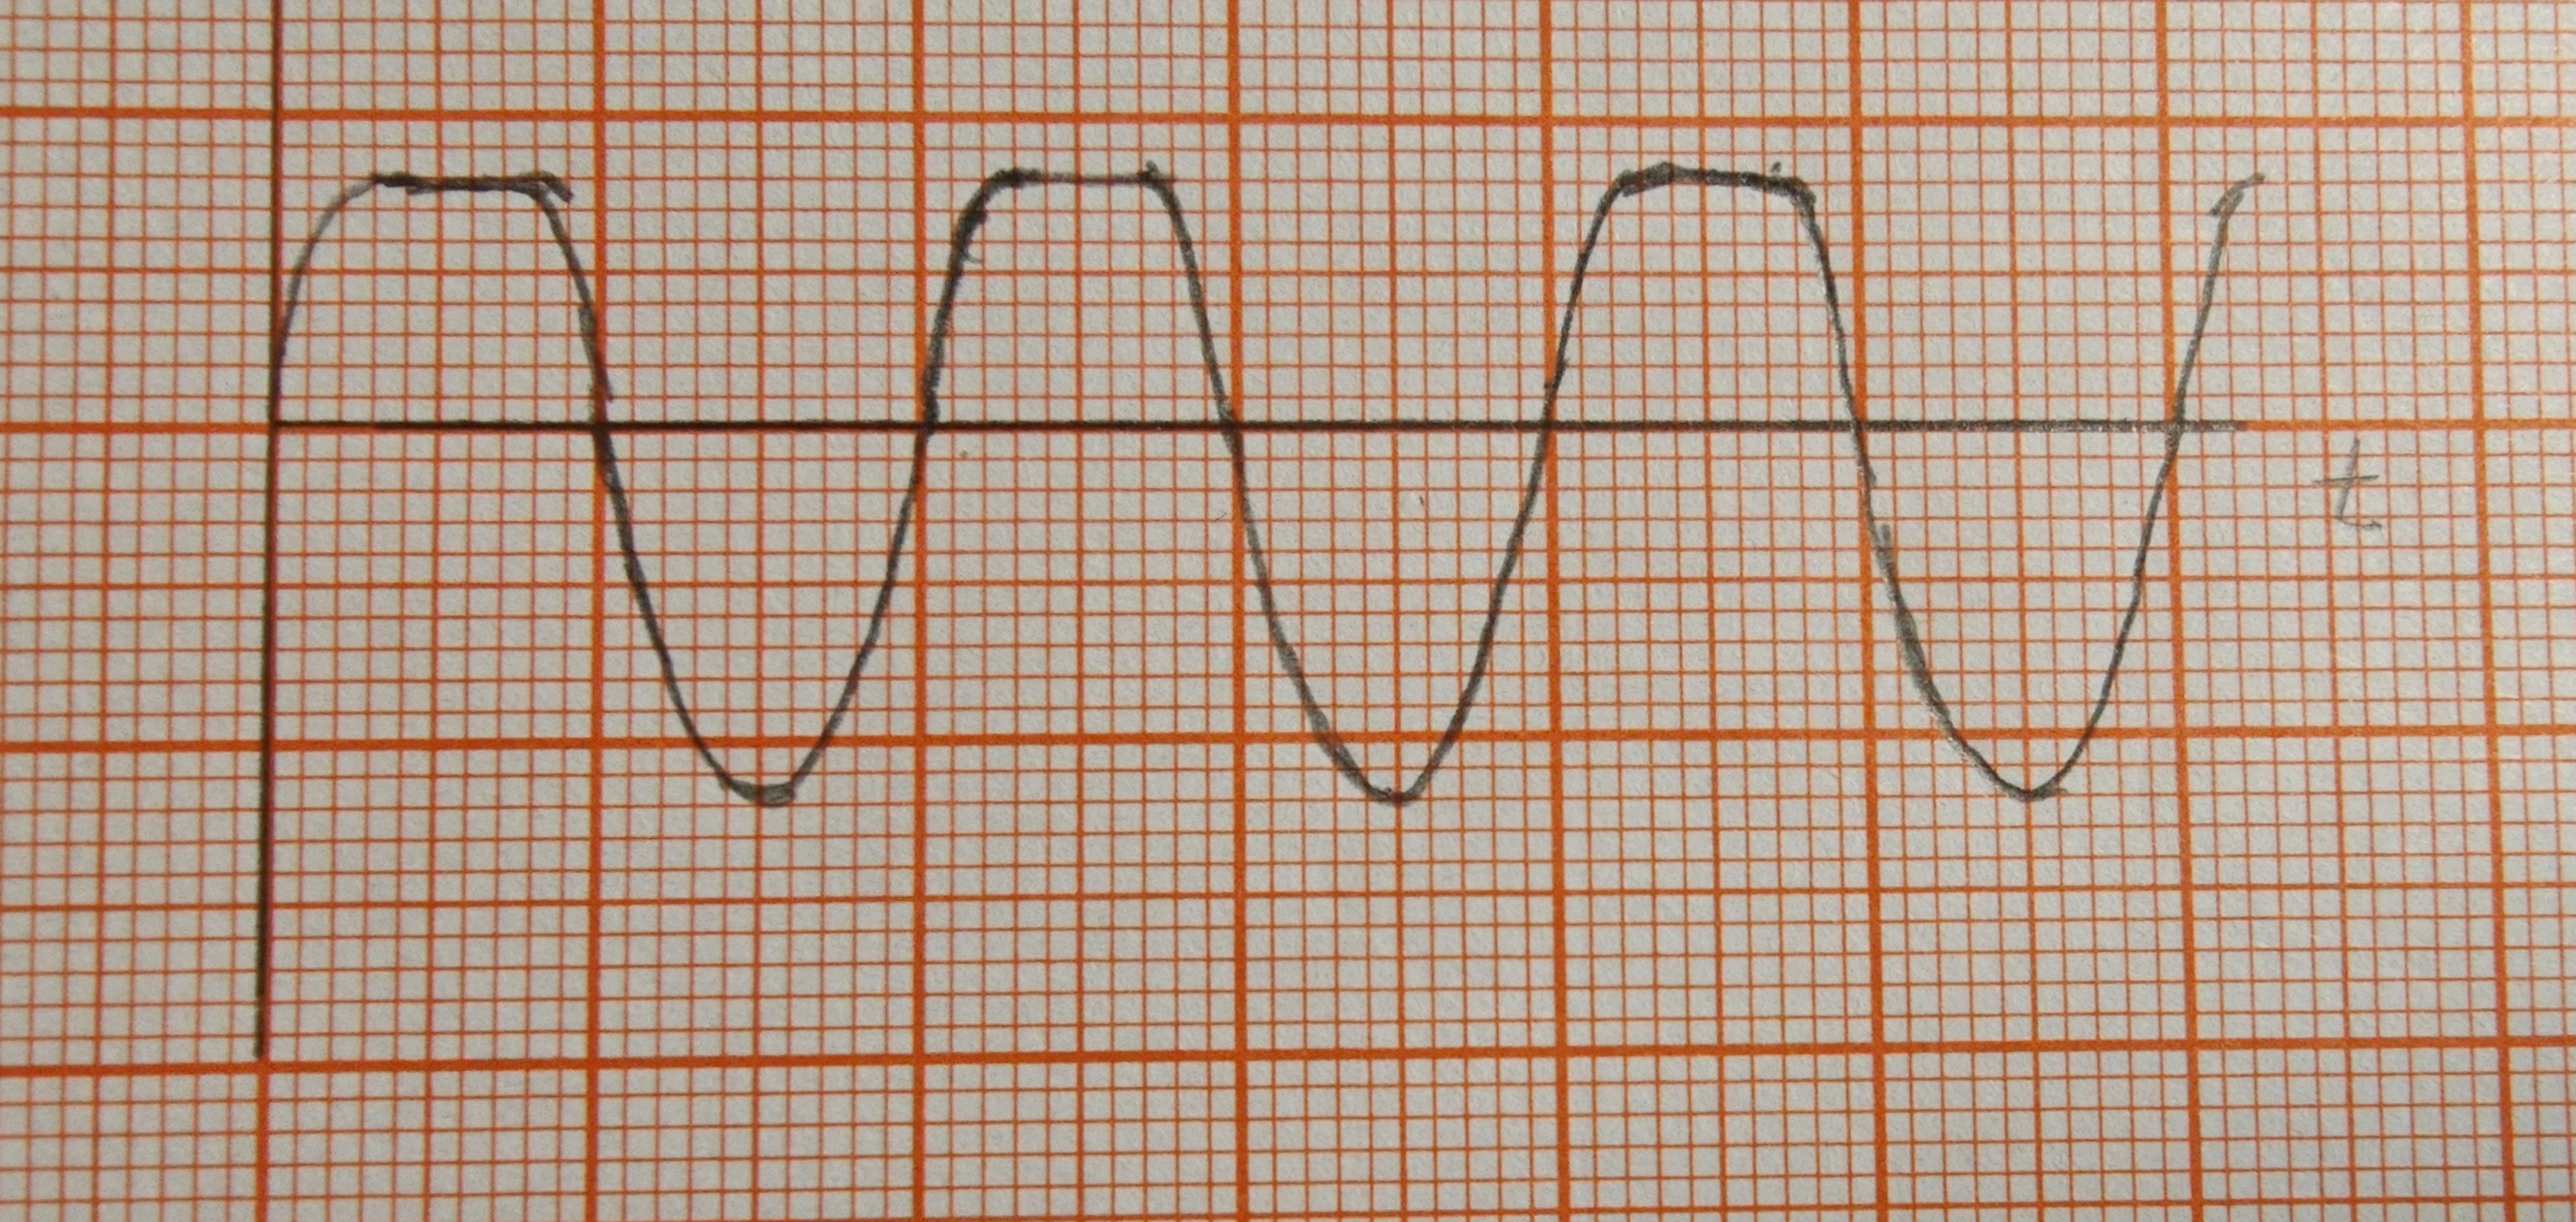
\includegraphics[width=0.48\textwidth]{2.20.jpg}
	}
\end{figure}

下表记录了失真时的静态工作点:

\begin{table}[h]
	\centering
	\caption{实测数据与计算结果}
	\begin{tabular}{|c|c|c|c|c|c|c|}
	\hline
	\( V_G/\mathrm{V} \) & \( V_S/\mathrm{V} \) & \( V_D/\mathrm{V} \) & \( I_{DQ} = \frac{V_S}{R_S} \) (mA) & \( V_{GSQ} = V_G - V_S \) (V) & \( V_{DSQ} = V_D - V_S \) (V) & 失真类型 \\
	\hline
	3.6575 & 1.9516 & 2.1942 & 1.9096 & 1.7059 & 0.2426 & 饱和失真 \\
	\hline
	1.6992 & 0.2055 & 10.9606 & 0.2011 & 1.4937 & 10.7551 & 截止失真 \\
	\hline
	\end{tabular}
\end{table}

\section{实验小结}

本次实验最大的感受是,仿真的结果与实验的结果差距非常大。更换一些元器件后结果仍然变化不大,实际上仿真与插板实验就是会有所不同。

这次实验中让我收获最大的是对Multisim电路仿真软件有了熟练的掌握,我基本学会了Multisim的仿真分析方式。

\end{document}